\documentclass[11pt,]{article}
\usepackage[left=1in,top=1in,right=1in,bottom=1in]{geometry}
\newcommand*{\authorfont}{\fontfamily{phv}\selectfont}
\usepackage[]{mathpazo}


  \usepackage[T1]{fontenc}
  \usepackage[utf8]{inputenc}



\usepackage{abstract}
\renewcommand{\abstractname}{}    % clear the title
\renewcommand{\absnamepos}{empty} % originally center

\renewenvironment{abstract}
 {{%
    \setlength{\leftmargin}{0mm}
    \setlength{\rightmargin}{\leftmargin}%
  }%
  \relax}
 {\endlist}

\makeatletter
\def\@maketitle{%
  \newpage
%  \null
%  \vskip 2em%
%  \begin{center}%
  \let \footnote \thanks
    {\fontsize{18}{20}\selectfont\raggedright  \setlength{\parindent}{0pt} \@title \par}%
}
%\fi
\makeatother




\setcounter{secnumdepth}{3}

\usepackage{color}
\usepackage{fancyvrb}
\newcommand{\VerbBar}{|}
\newcommand{\VERB}{\Verb[commandchars=\\\{\}]}
\DefineVerbatimEnvironment{Highlighting}{Verbatim}{commandchars=\\\{\}}
% Add ',fontsize=\small' for more characters per line
\usepackage{framed}
\definecolor{shadecolor}{RGB}{248,248,248}
\newenvironment{Shaded}{\begin{snugshade}}{\end{snugshade}}
\newcommand{\KeywordTok}[1]{\textcolor[rgb]{0.13,0.29,0.53}{\textbf{#1}}}
\newcommand{\DataTypeTok}[1]{\textcolor[rgb]{0.13,0.29,0.53}{#1}}
\newcommand{\DecValTok}[1]{\textcolor[rgb]{0.00,0.00,0.81}{#1}}
\newcommand{\BaseNTok}[1]{\textcolor[rgb]{0.00,0.00,0.81}{#1}}
\newcommand{\FloatTok}[1]{\textcolor[rgb]{0.00,0.00,0.81}{#1}}
\newcommand{\ConstantTok}[1]{\textcolor[rgb]{0.00,0.00,0.00}{#1}}
\newcommand{\CharTok}[1]{\textcolor[rgb]{0.31,0.60,0.02}{#1}}
\newcommand{\SpecialCharTok}[1]{\textcolor[rgb]{0.00,0.00,0.00}{#1}}
\newcommand{\StringTok}[1]{\textcolor[rgb]{0.31,0.60,0.02}{#1}}
\newcommand{\VerbatimStringTok}[1]{\textcolor[rgb]{0.31,0.60,0.02}{#1}}
\newcommand{\SpecialStringTok}[1]{\textcolor[rgb]{0.31,0.60,0.02}{#1}}
\newcommand{\ImportTok}[1]{#1}
\newcommand{\CommentTok}[1]{\textcolor[rgb]{0.56,0.35,0.01}{\textit{#1}}}
\newcommand{\DocumentationTok}[1]{\textcolor[rgb]{0.56,0.35,0.01}{\textbf{\textit{#1}}}}
\newcommand{\AnnotationTok}[1]{\textcolor[rgb]{0.56,0.35,0.01}{\textbf{\textit{#1}}}}
\newcommand{\CommentVarTok}[1]{\textcolor[rgb]{0.56,0.35,0.01}{\textbf{\textit{#1}}}}
\newcommand{\OtherTok}[1]{\textcolor[rgb]{0.56,0.35,0.01}{#1}}
\newcommand{\FunctionTok}[1]{\textcolor[rgb]{0.00,0.00,0.00}{#1}}
\newcommand{\VariableTok}[1]{\textcolor[rgb]{0.00,0.00,0.00}{#1}}
\newcommand{\ControlFlowTok}[1]{\textcolor[rgb]{0.13,0.29,0.53}{\textbf{#1}}}
\newcommand{\OperatorTok}[1]{\textcolor[rgb]{0.81,0.36,0.00}{\textbf{#1}}}
\newcommand{\BuiltInTok}[1]{#1}
\newcommand{\ExtensionTok}[1]{#1}
\newcommand{\PreprocessorTok}[1]{\textcolor[rgb]{0.56,0.35,0.01}{\textit{#1}}}
\newcommand{\AttributeTok}[1]{\textcolor[rgb]{0.77,0.63,0.00}{#1}}
\newcommand{\RegionMarkerTok}[1]{#1}
\newcommand{\InformationTok}[1]{\textcolor[rgb]{0.56,0.35,0.01}{\textbf{\textit{#1}}}}
\newcommand{\WarningTok}[1]{\textcolor[rgb]{0.56,0.35,0.01}{\textbf{\textit{#1}}}}
\newcommand{\AlertTok}[1]{\textcolor[rgb]{0.94,0.16,0.16}{#1}}
\newcommand{\ErrorTok}[1]{\textcolor[rgb]{0.64,0.00,0.00}{\textbf{#1}}}
\newcommand{\NormalTok}[1]{#1}

\usepackage{graphicx,grffile}
\makeatletter
\def\maxwidth{\ifdim\Gin@nat@width>\linewidth\linewidth\else\Gin@nat@width\fi}
\def\maxheight{\ifdim\Gin@nat@height>\textheight\textheight\else\Gin@nat@height\fi}
\makeatother
% Scale images if necessary, so that they will not overflow the page
% margins by default, and it is still possible to overwrite the defaults
% using explicit options in \includegraphics[width, height, ...]{}
\setkeys{Gin}{width=\maxwidth,height=\maxheight,keepaspectratio}

\title{Mi proyecto\\
Subtítulo\\
Subtítulo  }



\author{\Large Roberto Marte\vspace{0.05in} \newline\normalsize\emph{Estudiante, Universidad Autónoma de Santo Domingo (UASD)}  }


\date{}

\usepackage{titlesec}

\titleformat*{\section}{\normalsize\bfseries}
\titleformat*{\subsection}{\normalsize\itshape}
\titleformat*{\subsubsection}{\normalsize\itshape}
\titleformat*{\paragraph}{\normalsize\itshape}
\titleformat*{\subparagraph}{\normalsize\itshape}

\titlespacing{\section}
{0pt}{36pt}{0pt}
\titlespacing{\subsection}
{0pt}{36pt}{0pt}
\titlespacing{\subsubsection}
{0pt}{36pt}{0pt}





\newtheorem{hypothesis}{Hypothesis}
\usepackage{setspace}

\makeatletter
\@ifpackageloaded{hyperref}{}{%
\ifxetex
  \PassOptionsToPackage{hyphens}{url}\usepackage[setpagesize=false, % page size defined by xetex
              unicode=false, % unicode breaks when used with xetex
              xetex]{hyperref}
\else
  \PassOptionsToPackage{hyphens}{url}\usepackage[unicode=true]{hyperref}
\fi
}

\@ifpackageloaded{color}{
    \PassOptionsToPackage{usenames,dvipsnames}{color}
}{%
    \usepackage[usenames,dvipsnames]{color}
}
\makeatother
\hypersetup{breaklinks=true,
            bookmarks=true,
            pdfauthor={Roberto Marte (Estudiante, Universidad Autónoma de Santo Domingo (UASD))},
             pdfkeywords = {Precipitaciones},  
            pdftitle={Mi proyecto\\
Subtítulo\\
Subtítulo},
            colorlinks=true,
            citecolor=blue,
            urlcolor=blue,
            linkcolor=magenta,
            pdfborder={0 0 0}}
\urlstyle{same}  % don't use monospace font for urls

% set default figure placement to htbp
\makeatletter
\def\fps@figure{htbp}
\makeatother

\usepackage{pdflscape} \newcommand{\blandscape}{\begin{landscape}}
\newcommand{\elandscape}{\end{landscape}}


% add tightlist ----------
\providecommand{\tightlist}{%
\setlength{\itemsep}{0pt}\setlength{\parskip}{0pt}}

\begin{document}
	
% \pagenumbering{arabic}% resets `page` counter to 1 
%
% \maketitle

{% \usefont{T1}{pnc}{m}{n}
\setlength{\parindent}{0pt}
\thispagestyle{plain}
{\fontsize{18}{20}\selectfont\raggedright 
\maketitle  % title \par  

}

{
   \vskip 13.5pt\relax \normalsize\fontsize{11}{12} 
\textbf{\authorfont Roberto Marte} \hskip 15pt \emph{\small Estudiante, Universidad Autónoma de Santo Domingo (UASD)}   

}

}








\begin{abstract}

    \hbox{\vrule height .2pt width 39.14pc}

    \vskip 8.5pt % \small 

\noindent Mi resumen


\vskip 8.5pt \noindent \emph{Keywords}: Precipitaciones \par

    \hbox{\vrule height .2pt width 39.14pc}



\end{abstract}


\vskip 6.5pt


\noindent  \section{Introducción}\label{introducciuxf3n}

Preguntas de investigación o tema abordado.

\section{Metodología}\label{metodologuxeda}

\ldots

\section{Resultados}\label{resultados}

\ldots

\section{Discusión o Conclusiones}\label{discusiuxf3n-o-conclusiones}

\ldots

\section{Información de soporte}\label{informaciuxf3n-de-soporte}

\ldots

\section{\texorpdfstring{\emph{Script}
reproducible}{Script reproducible}}\label{script-reproducible}

\begin{Shaded}
\begin{Highlighting}[]
\KeywordTok{library}\NormalTok{(}\StringTok{`}\DataTypeTok{sf}\StringTok{`}\NormalTok{)}
\end{Highlighting}
\end{Shaded}

\begin{verbatim}
## Linking to GEOS 3.7.1, GDAL 2.4.2, PROJ 5.2.0
\end{verbatim}

\begin{Shaded}
\begin{Highlighting}[]
\KeywordTok{library}\NormalTok{(}\StringTok{`}\DataTypeTok{raster}\StringTok{`}\NormalTok{)}
\end{Highlighting}
\end{Shaded}

\begin{verbatim}
## Loading required package: sp
\end{verbatim}

\begin{Shaded}
\begin{Highlighting}[]
\KeywordTok{library}\NormalTok{(}\StringTok{`}\DataTypeTok{rgdal}\StringTok{`}\NormalTok{)}
\end{Highlighting}
\end{Shaded}

\begin{verbatim}
## rgdal: version: 1.4-6, (SVN revision 841)
##  Geospatial Data Abstraction Library extensions to R successfully loaded
##  Loaded GDAL runtime: GDAL 2.4.2, released 2019/06/28
##  Path to GDAL shared files: /usr/share/gdal
##  GDAL binary built with GEOS: TRUE 
##  Loaded PROJ.4 runtime: Rel. 5.2.0, September 15th, 2018, [PJ_VERSION: 520]
##  Path to PROJ.4 shared files: (autodetected)
##  Linking to sp version: 1.3-1
\end{verbatim}

\begin{Shaded}
\begin{Highlighting}[]
\KeywordTok{library}\NormalTok{(}\StringTok{`}\DataTypeTok{tidyverse}\StringTok{`}\NormalTok{)}
\end{Highlighting}
\end{Shaded}

\begin{verbatim}
## -- Attaching packages -------------------------------------------------------------- tidyverse 1.2.1 --
\end{verbatim}

\begin{verbatim}
## v ggplot2 3.2.1     v purrr   0.3.3
## v tibble  2.1.3     v dplyr   0.8.3
## v tidyr   1.0.0     v stringr 1.4.0
## v readr   1.3.1     v forcats 0.4.0
\end{verbatim}

\begin{verbatim}
## -- Conflicts ----------------------------------------------------------------- tidyverse_conflicts() --
## x tidyr::extract() masks raster::extract()
## x dplyr::filter()  masks stats::filter()
## x dplyr::lag()     masks stats::lag()
## x dplyr::select()  masks raster::select()
\end{verbatim}

\begin{Shaded}
\begin{Highlighting}[]
\KeywordTok{library}\NormalTok{(readxl)}
\KeywordTok{library}\NormalTok{(}\StringTok{`}\DataTypeTok{spdep}\StringTok{`}\NormalTok{)}
\end{Highlighting}
\end{Shaded}

\begin{verbatim}
## Loading required package: spData
\end{verbatim}

\begin{verbatim}
## To access larger datasets in this package, install the spDataLarge
## package with: `install.packages('spDataLarge',
## repos='https://nowosad.github.io/drat/', type='source')`
\end{verbatim}

\begin{Shaded}
\begin{Highlighting}[]
\KeywordTok{library}\NormalTok{(}\StringTok{`}\DataTypeTok{lmtest}\StringTok{`}\NormalTok{)}
\end{Highlighting}
\end{Shaded}

\begin{verbatim}
## Loading required package: zoo
\end{verbatim}

\begin{verbatim}
## 
## Attaching package: 'zoo'
\end{verbatim}

\begin{verbatim}
## The following objects are masked from 'package:base':
## 
##     as.Date, as.Date.numeric
\end{verbatim}

\begin{Shaded}
\begin{Highlighting}[]
\KeywordTok{library}\NormalTok{(}\StringTok{`}\DataTypeTok{tmap}\StringTok{`}\NormalTok{)}
\KeywordTok{library}\NormalTok{(}\StringTok{`}\DataTypeTok{RColorBrewer}\StringTok{`}\NormalTok{)}
\end{Highlighting}
\end{Shaded}

\subsubsection{Datos fuente}\label{datos-fuente}

Tomaremos como ejemplo la precipitación del año 1990. Primero carguemos
los observatorios y las provincias:

\begin{Shaded}
\begin{Highlighting}[]
\KeywordTok{library}\NormalTok{(sf)}
\NormalTok{rutapre <-}\StringTok{ 'data/onamet_prec_anual_sf.gpkg'}

\NormalTok{rutadiv <-}\StringTok{ 'data/divisionRD.gpkg'}
\KeywordTok{st_layers}\NormalTok{(rutapre)}
\end{Highlighting}
\end{Shaded}

\begin{verbatim}
## Driver: GPKG 
## Available layers:
##             layer_name geometry_type features fields
## 1 onamet_prec_anual_sf         Point       25     37
\end{verbatim}

\begin{Shaded}
\begin{Highlighting}[]
\NormalTok{pre <-}\StringTok{ }\KeywordTok{st_read}\NormalTok{(rutapre)}
\end{Highlighting}
\end{Shaded}

\begin{verbatim}
## Reading layer `onamet_prec_anual_sf' from data source `/home/rober/unidad-0-asignacion-99-mi-proyecto/data/onamet_prec_anual_sf.gpkg' using driver `GPKG'
## Simple feature collection with 25 features and 37 fields
## geometry type:  POINT
## dimension:      XY
## bbox:           xmin: -71.7 ymin: 18.067 xmax: -68.367 ymax: 19.85
## epsg (SRID):    4326
## proj4string:    +proj=longlat +datum=WGS84 +no_defs
\end{verbatim}

\begin{Shaded}
\begin{Highlighting}[]
\NormalTok{pre}
\end{Highlighting}
\end{Shaded}

\begin{verbatim}
## Simple feature collection with 25 features and 37 fields
## geometry type:  POINT
## dimension:      XY
## bbox:           xmin: -71.7 ymin: 18.067 xmax: -68.367 ymax: 19.85
## epsg (SRID):    4326
## proj4string:    +proj=longlat +datum=WGS84 +no_defs
## First 10 features:
##            Estación  a1979  a1980  a1981  a1982  a1983  a1984  a1985
## 1          Barahona 1740.0 1053.6 1435.3  815.3 1183.0  584.1  997.8
## 2         Bayaguana 2794.3 1761.5 2412.4 1758.6 1857.1 1645.6 1928.3
## 3           Cabrera 2035.0 1276.8     NA 2136.9 1703.8 1888.7 1557.1
## 4         Constanza 1652.1 1166.9 1343.3  921.2  828.4     NA  892.8
## 5  Gaspar Hernández     NA 1443.8 2174.9 1844.1 1688.8 2208.8 1895.5
## 6       Hondo Valle 1823.6 1778.2 2203.7 1709.9 1841.3 1796.6 1309.5
## 7            Jimaní 1060.7  639.1  960.2  507.5  610.7  641.5  689.6
## 8          La Unión 1781.5 1630.6 2304.4 1413.1 1288.4 1499.4 1157.1
## 9           La Vega 1833.5 1304.3 1993.7 1483.2 1353.9 1550.1 1084.9
## 10     Las Américas 1958.4  958.7 1513.4  787.4  975.5  954.9 1398.2
##     a1986  a1987  a1988  a1989   a1990  a1991  a1992  a1993  a1994   a1995
## 1  1080.0 1423.9  704.7 1011.6 1075.20  983.1 1112.5  968.5 1622.4  956.00
## 2  2182.2 2273.5 1813.2 1730.6 1823.40 1850.3 1765.7 1606.2 1892.8 1360.10
## 3  1597.0 2059.7     NA 1176.9 1183.40  957.6     NA     NA     NA      NA
## 4   715.8  786.9  837.7  671.5  875.35     NA  858.6  858.6  900.7  839.40
## 5  2874.7 2360.8 1426.3 1214.2 1530.70     NA 1257.5 1345.3 1824.9 1665.45
## 6  1589.7 1778.8 1766.5 1722.8 1596.10 1088.4 1731.0 1887.0 1772.0 1288.30
## 7   802.4  648.9  521.0  680.7  880.00  311.6  809.2  472.9  840.2  909.00
## 8  1313.1 1786.5 1888.8 1222.8 1808.00 1250.4 1555.2 1484.8 1035.9  877.70
## 9  1767.1 1663.2 1934.9 1192.4 1664.40 1146.4 1565.6 1855.4 1455.7 1175.40
## 10 1419.0 1866.4 1620.5 1151.7      NA  997.0     NA     NA     NA 1017.50
##      a1996   a1997  a1998  a1999  a2000  a2001  a2002   a2003  a2004
## 1   965.65  662.60  684.6  662.7  600.0  600.0  997.6  942.60  972.6
## 2  1867.70 1618.60 2156.6 1712.5 1868.5 1796.1 1658.0 2117.30 1554.2
## 3       NA      NA     NA     NA 1538.6 1852.9  946.9 1810.95 2053.3
## 4  1167.30  525.10 1492.7 1077.8  951.3  787.1  959.2 1084.10  985.9
## 5  2656.80  984.80 2147.9 1791.9 1716.9 2178.8 1093.4 2058.50 1906.8
## 6  1447.90  912.65 1813.9 1762.2 2285.9 1604.3 1477.4 1628.10 1617.7
## 7   816.20  358.20  824.1 1037.0  833.9  488.4  510.1  656.70  866.9
## 8  1980.50  554.20 1744.1 1314.3 1148.5 1360.5  972.1 1802.00 2550.1
## 9  1772.50 1018.80 1549.6 1817.9 1368.6 1522.0 1200.7 2290.60 1825.7
## 10 1019.60  651.20 1218.6 1125.9  809.7  747.6  933.4 1083.60 1338.9
##      a2005   a2006   a2007   a2008  a2009  a2010  a2011  a2012  a2013
## 1  1274.60 1118.40 1531.30 1136.80  583.3 1036.3 1280.2 1726.3  576.2
## 2  2102.80 2097.10 2137.60 1831.20 1607.9 1881.6 1849.9 2350.8 2108.0
## 3  1451.10 1957.90      NA      NA     NA 2411.4 1920.1 2821.3     NA
## 4  1245.20 1162.20 1661.40 1072.90  902.8 1024.5 1008.2 1188.1 1016.3
## 5  2001.85 1992.00 3282.65 1866.30 2386.1 2639.2 1727.2 2524.0 1448.2
## 6  1554.65 1487.15 1487.15 1399.15 1461.9 2005.6 1309.0 1736.8 1390.2
## 7   929.30  963.90 1084.00  751.10  694.9  807.1  879.5 1037.3  292.9
## 8  2034.30 2106.60 2764.80 1536.30 1605.8 2255.6 1719.2 2484.3 1299.2
## 9  1245.20 1162.20 1661.40 1072.90 2867.4 1486.4 1434.1 2204.7 1227.0
## 10 1744.60 1141.70 1457.50 1718.40 1369.1 2422.4 1885.5 1658.7 1039.6
##     a2014                    geom
## 1   845.9      POINT (-71.1 18.2)
## 2  1505.6 POINT (-69.63333 18.75)
## 3  1975.6    POINT (-69.9 19.633)
## 4   764.1      POINT (-70.7 18.9)
## 5  1928.7    POINT (-70.3 19.617)
## 6   908.9    POINT (-71.7 18.717)
## 7   502.0  POINT (-71.633 18.483)
## 8  1741.5    POINT (-70.55 19.75)
## 9  1812.5  POINT (-70.533 19.217)
## 10  909.4  POINT (-69.667 18.433)
\end{verbatim}

\begin{Shaded}
\begin{Highlighting}[]
\KeywordTok{st_layers}\NormalTok{(rutadiv)}
\end{Highlighting}
\end{Shaded}

\begin{verbatim}
## Driver: GPKG 
## Available layers:
##      layer_name geometry_type features fields
## 1 PROVCenso2010       Polygon       32      4
## 2  MUNCenso2010       Polygon      155      5
## 3  REGCenso2010       Polygon       10      2
\end{verbatim}

\begin{Shaded}
\begin{Highlighting}[]
\NormalTok{prov <-}\StringTok{ }\KeywordTok{st_read}\NormalTok{(rutadiv, }\DataTypeTok{layer =} \StringTok{'PROVCenso2010'}\NormalTok{)}
\end{Highlighting}
\end{Shaded}

\begin{verbatim}
## Reading layer `PROVCenso2010' from data source `/home/rober/unidad-0-asignacion-99-mi-proyecto/data/divisionRD.gpkg' using driver `GPKG'
## Simple feature collection with 32 features and 4 fields
## geometry type:  MULTIPOLYGON
## dimension:      XY
## bbox:           xmin: 182215.8 ymin: 1933532 xmax: 571365.3 ymax: 2205216
## epsg (SRID):    32619
## proj4string:    +proj=utm +zone=19 +datum=WGS84 +units=m +no_defs
\end{verbatim}

\begin{Shaded}
\begin{Highlighting}[]
\NormalTok{prov}
\end{Highlighting}
\end{Shaded}

\begin{verbatim}
## Simple feature collection with 32 features and 4 fields
## geometry type:  MULTIPOLYGON
## dimension:      XY
## bbox:           xmin: 182215.8 ymin: 1933532 xmax: 571365.3 ymax: 2205216
## epsg (SRID):    32619
## proj4string:    +proj=utm +zone=19 +datum=WGS84 +units=m +no_defs
## First 10 features:
##    PROV REG         TOPONIMIA ENLACE                           geom
## 1    01  10 DISTRITO NACIONAL   1001 MULTIPOLYGON (((406845.9 20...
## 2    02  05              AZUA   0502 MULTIPOLYGON (((322129.5 20...
## 3    03  06           BAORUCO   0603 MULTIPOLYGON (((271940 2060...
## 4    04  06          BARAHONA   0604 MULTIPOLYGON (((291856.5 20...
## 5    05  04           DAJABÓN   0405 MULTIPOLYGON (((245433.3 21...
## 6    06  03            DUARTE   0306 MULTIPOLYGON (((374434.8 21...
## 7    07  07        ELÍAS PIÑA   0707 MULTIPOLYGON (((235630.8 21...
## 8    08  08          EL SEIBO   0808 MULTIPOLYGON (((523436.4 20...
## 9    09  01         ESPAILLAT   0109 MULTIPOLYGON (((385993.5 21...
## 10   10  06     INDEPENDENCIA   0610 MULTIPOLYGON (((205698.2 20...
\end{verbatim}

Exploremos el CRS del objeto \texttt{obs}.

\begin{Shaded}
\begin{Highlighting}[]
\KeywordTok{st_crs}\NormalTok{(pre)}
\end{Highlighting}
\end{Shaded}

\begin{verbatim}
## Coordinate Reference System:
##   EPSG: 4326 
##   proj4string: "+proj=longlat +datum=WGS84 +no_defs"
\end{verbatim}

Transformemos a 32619:

\begin{Shaded}
\begin{Highlighting}[]
\NormalTok{crsdestino <-}\StringTok{ }\DecValTok{32619}
\NormalTok{preutm <-}\StringTok{ }\NormalTok{pre }\OperatorTok\StringTok{ }\KeywordTok{st_transform}\NormalTok{(}\DataTypeTok{crs =}\NormalTok{ crsdestino)}
\NormalTok{preutm}
\end{Highlighting}
\end{Shaded}

\begin{verbatim}
## Simple feature collection with 25 features and 37 fields
## geometry type:  POINT
## dimension:      XY
## bbox:           xmin: 215264.1 ymin: 1999092 xmax: 566794.7 ymax: 2197035
## epsg (SRID):    32619
## proj4string:    +proj=utm +zone=19 +datum=WGS84 +units=m +no_defs
## First 10 features:
##            Estación  a1979  a1980  a1981  a1982  a1983  a1984  a1985
## 1          Barahona 1740.0 1053.6 1435.3  815.3 1183.0  584.1  997.8
## 2         Bayaguana 2794.3 1761.5 2412.4 1758.6 1857.1 1645.6 1928.3
## 3           Cabrera 2035.0 1276.8     NA 2136.9 1703.8 1888.7 1557.1
## 4         Constanza 1652.1 1166.9 1343.3  921.2  828.4     NA  892.8
## 5  Gaspar Hernández     NA 1443.8 2174.9 1844.1 1688.8 2208.8 1895.5
## 6       Hondo Valle 1823.6 1778.2 2203.7 1709.9 1841.3 1796.6 1309.5
## 7            Jimaní 1060.7  639.1  960.2  507.5  610.7  641.5  689.6
## 8          La Unión 1781.5 1630.6 2304.4 1413.1 1288.4 1499.4 1157.1
## 9           La Vega 1833.5 1304.3 1993.7 1483.2 1353.9 1550.1 1084.9
## 10     Las Américas 1958.4  958.7 1513.4  787.4  975.5  954.9 1398.2
##     a1986  a1987  a1988  a1989   a1990  a1991  a1992  a1993  a1994   a1995
## 1  1080.0 1423.9  704.7 1011.6 1075.20  983.1 1112.5  968.5 1622.4  956.00
## 2  2182.2 2273.5 1813.2 1730.6 1823.40 1850.3 1765.7 1606.2 1892.8 1360.10
## 3  1597.0 2059.7     NA 1176.9 1183.40  957.6     NA     NA     NA      NA
## 4   715.8  786.9  837.7  671.5  875.35     NA  858.6  858.6  900.7  839.40
## 5  2874.7 2360.8 1426.3 1214.2 1530.70     NA 1257.5 1345.3 1824.9 1665.45
## 6  1589.7 1778.8 1766.5 1722.8 1596.10 1088.4 1731.0 1887.0 1772.0 1288.30
## 7   802.4  648.9  521.0  680.7  880.00  311.6  809.2  472.9  840.2  909.00
## 8  1313.1 1786.5 1888.8 1222.8 1808.00 1250.4 1555.2 1484.8 1035.9  877.70
## 9  1767.1 1663.2 1934.9 1192.4 1664.40 1146.4 1565.6 1855.4 1455.7 1175.40
## 10 1419.0 1866.4 1620.5 1151.7      NA  997.0     NA     NA     NA 1017.50
##      a1996   a1997  a1998  a1999  a2000  a2001  a2002   a2003  a2004
## 1   965.65  662.60  684.6  662.7  600.0  600.0  997.6  942.60  972.6
## 2  1867.70 1618.60 2156.6 1712.5 1868.5 1796.1 1658.0 2117.30 1554.2
## 3       NA      NA     NA     NA 1538.6 1852.9  946.9 1810.95 2053.3
## 4  1167.30  525.10 1492.7 1077.8  951.3  787.1  959.2 1084.10  985.9
## 5  2656.80  984.80 2147.9 1791.9 1716.9 2178.8 1093.4 2058.50 1906.8
## 6  1447.90  912.65 1813.9 1762.2 2285.9 1604.3 1477.4 1628.10 1617.7
## 7   816.20  358.20  824.1 1037.0  833.9  488.4  510.1  656.70  866.9
## 8  1980.50  554.20 1744.1 1314.3 1148.5 1360.5  972.1 1802.00 2550.1
## 9  1772.50 1018.80 1549.6 1817.9 1368.6 1522.0 1200.7 2290.60 1825.7
## 10 1019.60  651.20 1218.6 1125.9  809.7  747.6  933.4 1083.60 1338.9
##      a2005   a2006   a2007   a2008  a2009  a2010  a2011  a2012  a2013
## 1  1274.60 1118.40 1531.30 1136.80  583.3 1036.3 1280.2 1726.3  576.2
## 2  2102.80 2097.10 2137.60 1831.20 1607.9 1881.6 1849.9 2350.8 2108.0
## 3  1451.10 1957.90      NA      NA     NA 2411.4 1920.1 2821.3     NA
## 4  1245.20 1162.20 1661.40 1072.90  902.8 1024.5 1008.2 1188.1 1016.3
## 5  2001.85 1992.00 3282.65 1866.30 2386.1 2639.2 1727.2 2524.0 1448.2
## 6  1554.65 1487.15 1487.15 1399.15 1461.9 2005.6 1309.0 1736.8 1390.2
## 7   929.30  963.90 1084.00  751.10  694.9  807.1  879.5 1037.3  292.9
## 8  2034.30 2106.60 2764.80 1536.30 1605.8 2255.6 1719.2 2484.3 1299.2
## 9  1245.20 1162.20 1661.40 1072.90 2867.4 1486.4 1434.1 2204.7 1227.0
## 10 1744.60 1141.70 1457.50 1718.40 1369.1 2422.4 1885.5 1658.7 1039.6
##     a2014                     geom
## 1   845.9 POINT (277900.2 2013585)
## 2  1505.6 POINT (433242.1 2073284)
## 3  1975.6   POINT (405636 2171119)
## 4   764.1 POINT (320947.7 2090623)
## 5  1928.7 POINT (363678.2 2169619)
## 6   908.9 POINT (215264.1 2071669)
## 7   502.0 POINT (221953.7 2045651)
## 8  1741.5 POINT (337592.1 2184559)
## 9  1812.5 POINT (338847.1 2125548)
## 10  909.4 POINT (429562.7 2038222)
\end{verbatim}

\subsubsection{EDA básico}\label{eda-buxe1sico}

Obtengamos los estadísticos básicos para el año 1990:

\begin{Shaded}
\begin{Highlighting}[]
\KeywordTok{nrow}\NormalTok{(preutm)}
\end{Highlighting}
\end{Shaded}

\begin{verbatim}
## [1] 25
\end{verbatim}

\begin{Shaded}
\begin{Highlighting}[]
\KeywordTok{summary}\NormalTok{(preutm}\OperatorTok{$}\NormalTok{a1990)}
\end{Highlighting}
\end{Shaded}

\begin{verbatim}
##    Min. 1st Qu.  Median    Mean 3rd Qu.    Max.    NA's 
##   512.8  1035.8  1472.5  1401.1  1700.3  2261.2       1
\end{verbatim}

\begin{Shaded}
\begin{Highlighting}[]
\KeywordTok{hist}\NormalTok{(preutm}\OperatorTok{$}\NormalTok{a1990)}
\end{Highlighting}
\end{Shaded}

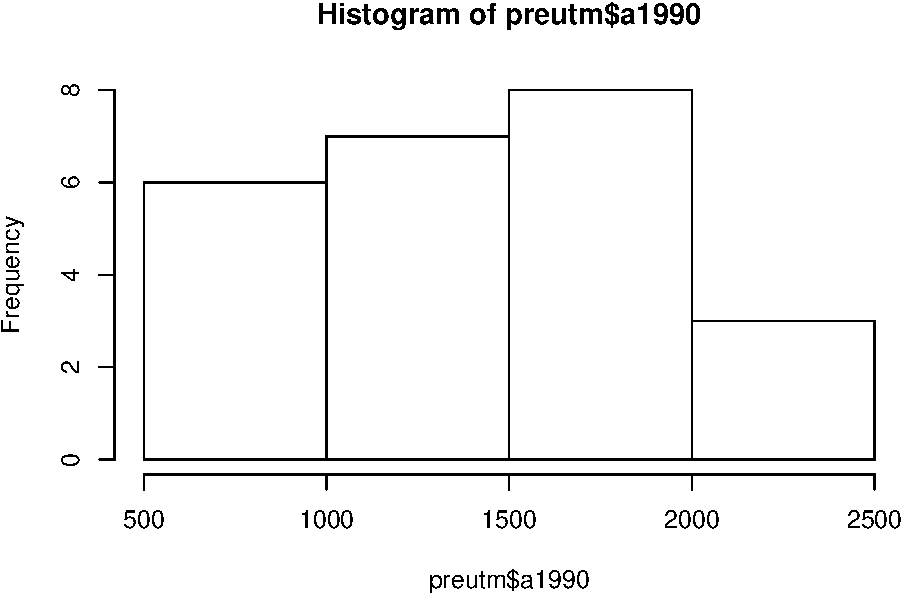
\includegraphics[width=600px]{Proyecto-Precipitaciones_files/figure-latex/esda-1990-1}

\begin{Shaded}
\begin{Highlighting}[]
\KeywordTok{hist}\NormalTok{(}\KeywordTok{log}\NormalTok{(preutm}\OperatorTok{$}\NormalTok{a1990))}
\end{Highlighting}
\end{Shaded}

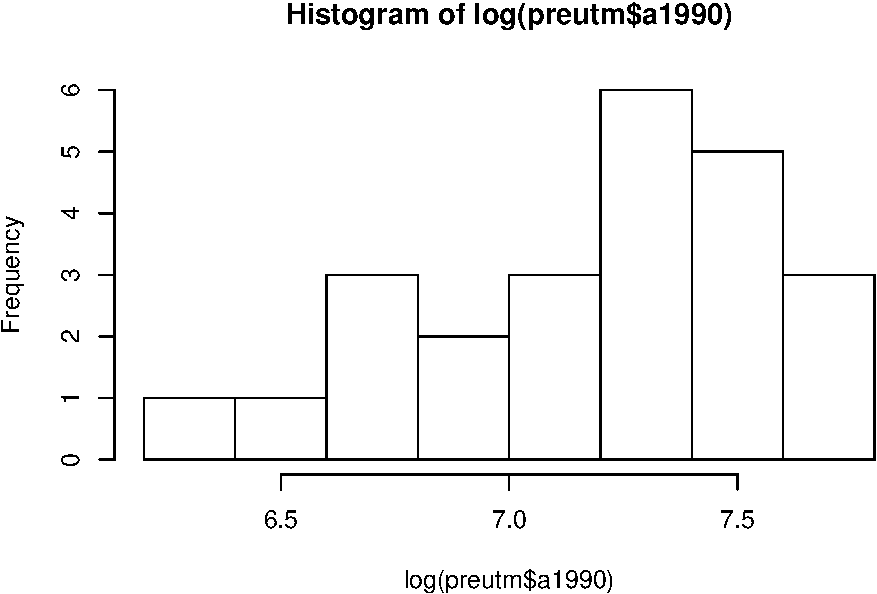
\includegraphics[width=600px]{Proyecto-Precipitaciones_files/figure-latex/esda-1990-2}

\begin{Shaded}
\begin{Highlighting}[]
\KeywordTok{shapiro.test}\NormalTok{(preutm}\OperatorTok{$}\NormalTok{a1990)}
\end{Highlighting}
\end{Shaded}

\begin{verbatim}
## 
##  Shapiro-Wilk normality test
## 
## data:  preutm$a1990
## W = 0.9728, p-value = 0.7362
\end{verbatim}

\begin{Shaded}
\begin{Highlighting}[]
\KeywordTok{shapiro.test}\NormalTok{(}\KeywordTok{log}\NormalTok{(pre}\OperatorTok{$}\NormalTok{a1990))}
\end{Highlighting}
\end{Shaded}

\begin{verbatim}
## 
##  Shapiro-Wilk normality test
## 
## data:  log(pre$a1990)
## W = 0.94861, p-value = 0.2527
\end{verbatim}

Como vemos, los datos siguen distribución normal, pero hay algo de sesgo
hacia la derecha en la distribución. Igualmente, de los 25 observatorios
que hay en todo el país, para 1979 en al menos 4 hay datos perdidos
(\texttt{NA}). Eliminemos dichos observatorios, generemos un objeto que
incluya solamente a 1979 y que contenga igualmente una columna con datos
transformados:

\begin{Shaded}
\begin{Highlighting}[]
\NormalTok{pre1990 <-}\StringTok{ }\KeywordTok{na.omit}\NormalTok{(preutm[,}\KeywordTok{c}\NormalTok{(}\StringTok{'Estación', '}\NormalTok{a1990}\StringTok{')])}
\StringTok{pre1990$a1990log <- log(pre1990$a1990)}
\StringTok{pre1990}
\end{Highlighting}
\end{Shaded}

\begin{verbatim}
## Simple feature collection with 24 features and 3 fields
## geometry type:  POINT
## dimension:      XY
## bbox:           xmin: 215264.1 ymin: 1999092 xmax: 566794.7 ymax: 2197035
## epsg (SRID):    32619
## proj4string:    +proj=utm +zone=19 +datum=WGS84 +units=m +no_defs
## First 10 features:
##            Estación   a1990                     geom a1990log
## 1          Barahona 1075.20 POINT (277900.2 2013585) 6.980262
## 2         Bayaguana 1823.40 POINT (433242.1 2073284) 7.508458
## 3           Cabrera 1183.40   POINT (405636 2171119) 7.076147
## 4         Constanza  875.35 POINT (320947.7 2090623) 6.774624
## 5  Gaspar Hernández 1530.70 POINT (363678.2 2169619) 7.333480
## 6       Hondo Valle 1596.10 POINT (215264.1 2071669) 7.375318
## 7            Jimaní  880.00 POINT (221953.7 2045651) 6.779922
## 8          La Unión 1808.00 POINT (337592.1 2184559) 7.499977
## 9           La Vega 1664.40 POINT (338847.1 2125548) 7.417220
## 11             Moca 1639.50 POINT (342475.8 2143891) 7.402147
\end{verbatim}

Representemos los observatorios, estilizando por tono según la
precipitación del año 1990:

\begin{Shaded}
\begin{Highlighting}[]
\KeywordTok{library}\NormalTok{(sp)}
\KeywordTok{library}\NormalTok{(ggplot2)}
\KeywordTok{ggplot}\NormalTok{() }\OperatorTok{+}
\StringTok{  }\KeywordTok{geom_sf}\NormalTok{(}\DataTypeTok{data =}\NormalTok{ prov, }\DataTypeTok{fill =} \StringTok{'white'}\NormalTok{) }\OperatorTok{+}
\StringTok{  }\KeywordTok{geom_sf}\NormalTok{(}\DataTypeTok{data =}\NormalTok{ pre1990, }\KeywordTok{aes}\NormalTok{(}\DataTypeTok{col =}\NormalTok{ a1990log), }\DataTypeTok{size =} \DecValTok{6}\NormalTok{) }\OperatorTok{+}
\StringTok{  }\KeywordTok{scale_colour_gradient}\NormalTok{(}\DataTypeTok{low=}\StringTok{"#deebf7"}\NormalTok{, }\DataTypeTok{high=}\StringTok{"#3182bd"}\NormalTok{) }\OperatorTok{+}
\StringTok{  }\KeywordTok{geom_sf_text}\NormalTok{(}\DataTypeTok{data =}\NormalTok{ prov, }\KeywordTok{aes}\NormalTok{(}\DataTypeTok{label=}\NormalTok{TOPONIMIA), }\DataTypeTok{check_overlap =}\NormalTok{ T, }\DataTypeTok{size =} \DecValTok{2}\NormalTok{) }\OperatorTok{+}
\StringTok{  }\KeywordTok{geom_sf_text}\NormalTok{(}\DataTypeTok{data =}\NormalTok{ pre1990, }\KeywordTok{aes}\NormalTok{(}\DataTypeTok{label=}\NormalTok{Estación), }\DataTypeTok{check_overlap =}\NormalTok{ T, }\DataTypeTok{size =} \FloatTok{1.5}\NormalTok{) }\OperatorTok{+}
\StringTok{  }\KeywordTok{theme_bw}\NormalTok{()}
\end{Highlighting}
\end{Shaded}

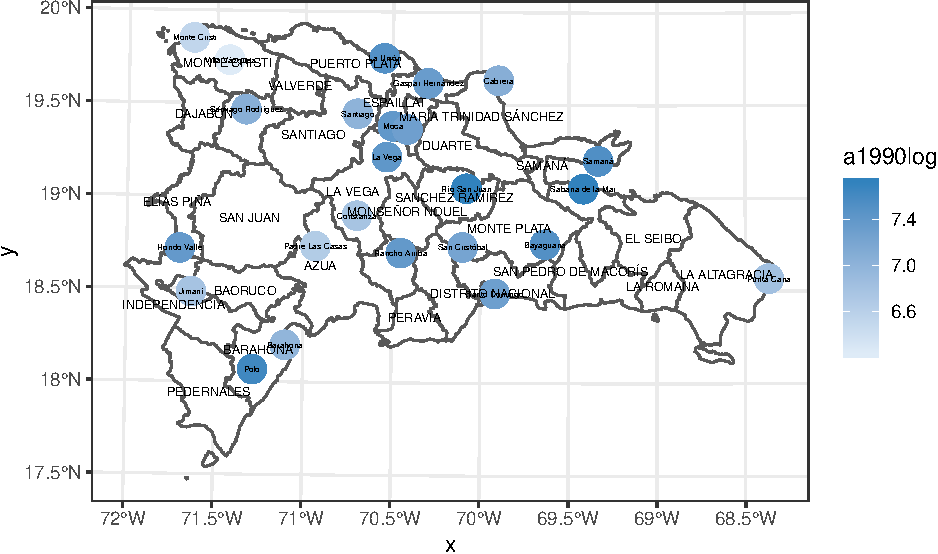
\includegraphics{Proyecto-Precipitaciones_files/figure-latex/mapa-pre-1990-1.pdf}

\subsubsection{Variograma muestral}\label{variograma-muestral}

Generemos el variograma muestral para el logaritmo de la precipitación.
Para ello empleamos la función \texttt{variogram}.

\begin{Shaded}
\begin{Highlighting}[]
\KeywordTok{library}\NormalTok{(sp)}
\KeywordTok{library}\NormalTok{(gstat)}
\end{Highlighting}
\end{Shaded}

\begin{verbatim}
## Registered S3 method overwritten by 'xts':
##   method     from
##   as.zoo.xts zoo
\end{verbatim}

\begin{Shaded}
\begin{Highlighting}[]
\KeywordTok{library}\NormalTok{(nlme)}
\end{Highlighting}
\end{Shaded}

\begin{verbatim}
## 
## Attaching package: 'nlme'
\end{verbatim}

\begin{verbatim}
## The following object is masked from 'package:dplyr':
## 
##     collapse
\end{verbatim}

\begin{verbatim}
## The following object is masked from 'package:raster':
## 
##     getData
\end{verbatim}

\begin{Shaded}
\begin{Highlighting}[]
\NormalTok{v90 <-}\StringTok{ }\KeywordTok{variogram}\NormalTok{(a1990log}\OperatorTok{~}\DecValTok{1}\NormalTok{, pre1990)}
\NormalTok{v90}
\end{Highlighting}
\end{Shaded}

\begin{verbatim}
##    np       dist       gamma dir.hor dir.ver   id
## 1   1   8896.559 0.006502436       0       0 var1
## 2   7  22355.182 0.076881026       0       0 var1
## 3  10  32118.137 0.080358606       0       0 var1
## 4   8  40371.385 0.055545000       0       0 var1
## 5   7  50078.452 0.092248889       0       0 var1
## 6  13  59038.478 0.072054740       0       0 var1
## 7  12  67482.051 0.115988337       0       0 var1
## 8   8  77729.231 0.064197043       0       0 var1
## 9  21  85220.747 0.122284553       0       0 var1
## 10 11  93434.242 0.197998092       0       0 var1
## 11 11 103535.175 0.105959793       0       0 var1
## 12 19 112257.676 0.189461155       0       0 var1
## 13 17 119969.781 0.137926928       0       0 var1
## 14 12 128732.245 0.103352130       0       0 var1
\end{verbatim}

\begin{Shaded}
\begin{Highlighting}[]
\KeywordTok{plot}\NormalTok{(v90, }\DataTypeTok{plot.numbers =}\NormalTok{ T)}
\end{Highlighting}
\end{Shaded}

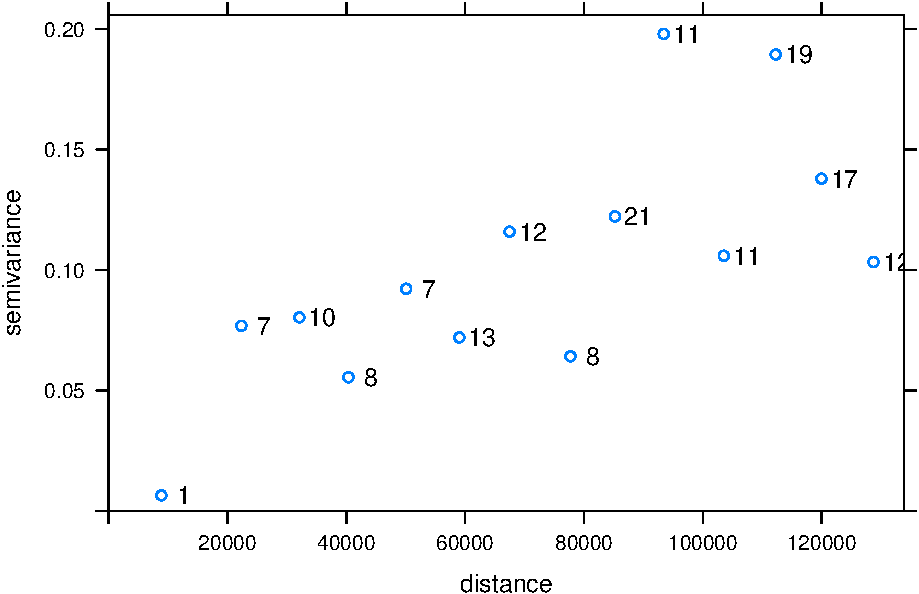
\includegraphics[width=800px]{Proyecto-Precipitaciones_files/figure-latex/vgm-pre1990-1}

Nótese la fórmula \texttt{a1990log\textasciitilde{}1}, la cual indica
que la precipitación de 1990 es la variable sobre la cual se generará el
variograma contra un modelo de media, que en este caso es simplemente un
intercepto (media desconocida y constante). Típicamente, este variograma
servirá para realizar un kriging ordinario.

La función \texttt{variogram} fija una distancia máxima de búsqueda
(\texttt{cutoff}), que equivale a un tercio de la diagonal del recuadro
delimitador (\emph{bounding box}), y fija intervalos de anchura
constante (\texttt{width}, que es la distancia de los intervalos
\emph{hi}, referida anteriormente) equivalentes a \texttt{cutoff/15}.
Dichos parámetros, \texttt{cutoff} y \texttt{width} pueden modificarse
por argumentos dentro de la función \texttt{variogram}.

\subsubsection{Variograma modelo}\label{variograma-modelo}

A partir del variograma muestral, generamos un variograma modelo que
será el que utlizará la función \texttt{krige} para realizar la
interpolación. Probamos varias opciones en función de lo visto en el
variograma muestral.

\begin{Shaded}
\begin{Highlighting}[]
\NormalTok{v90_m <-}\StringTok{ }\KeywordTok{fit.variogram}\NormalTok{(v90, }\KeywordTok{vgm}\NormalTok{(}\DataTypeTok{model =} \StringTok{"Sph"}\NormalTok{, }\DataTypeTok{range =} \DecValTok{50000}\NormalTok{))}
\NormalTok{v90_m}
\end{Highlighting}
\end{Shaded}

\begin{verbatim}
##   model     psill    range
## 1   Sph 0.1362796 97596.52
\end{verbatim}

\begin{Shaded}
\begin{Highlighting}[]
\KeywordTok{plot}\NormalTok{(v90, v90_m, }\DataTypeTok{plot.numbers =}\NormalTok{ T)}
\end{Highlighting}
\end{Shaded}

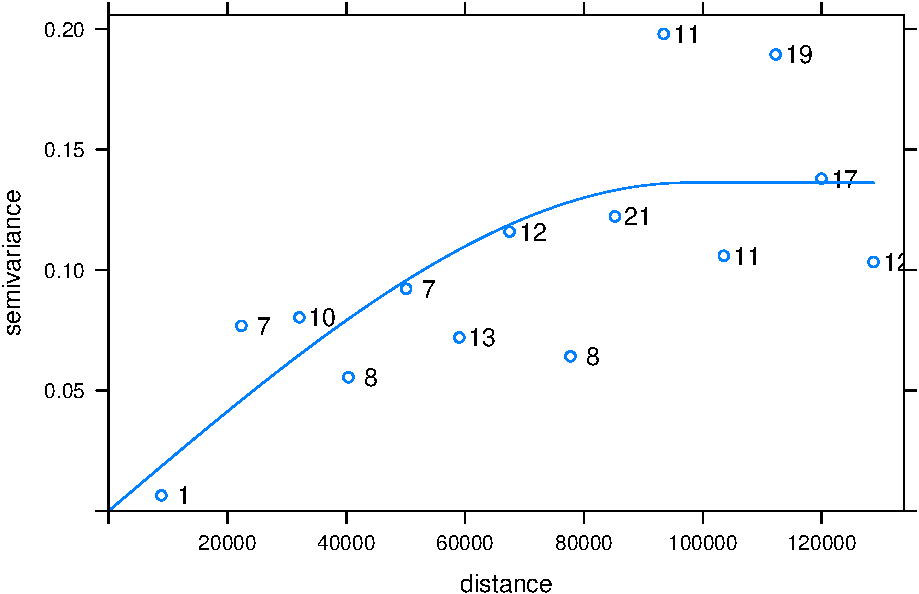
\includegraphics[width=800px]{Proyecto-Precipitaciones_files/figure-latex/vgm-pre1990-ajus-exp-1}

\begin{Shaded}
\begin{Highlighting}[]
\NormalTok{v90_m2 <-}\StringTok{ }\KeywordTok{fit.variogram}\NormalTok{(v90, }\KeywordTok{vgm}\NormalTok{(}\DataTypeTok{model =} \StringTok{"Exp"}\NormalTok{, }\DataTypeTok{range =} \DecValTok{50000}\NormalTok{))}
\NormalTok{v90_m2}
\end{Highlighting}
\end{Shaded}

\begin{verbatim}
##   model     psill    range
## 1   Exp 0.1511372 50116.48
\end{verbatim}

\begin{Shaded}
\begin{Highlighting}[]
\KeywordTok{plot}\NormalTok{(v90, v90_m2, }\DataTypeTok{plot.numbers =}\NormalTok{ T)}
\end{Highlighting}
\end{Shaded}

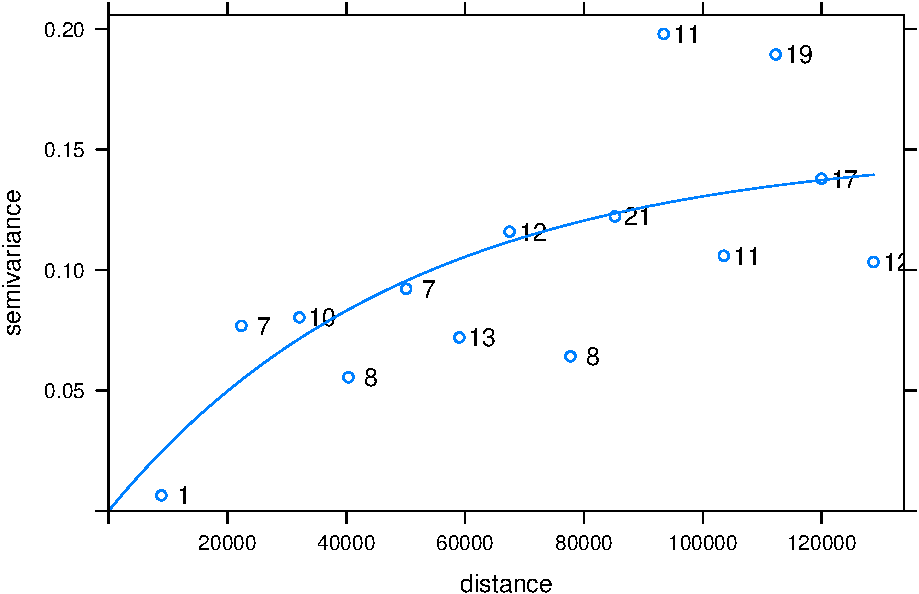
\includegraphics[width=800px]{Proyecto-Precipitaciones_files/figure-latex/vgm-pre1990-ajus-exp-2}

\begin{Shaded}
\begin{Highlighting}[]
\NormalTok{v90_m3 <-}\StringTok{ }\KeywordTok{fit.variogram}\NormalTok{(v90, }\KeywordTok{vgm}\NormalTok{(}\DataTypeTok{model =} \StringTok{"Gau"}\NormalTok{, }\DataTypeTok{range =} \DecValTok{50000}\NormalTok{))}
\NormalTok{v90_m3}
\end{Highlighting}
\end{Shaded}

\begin{verbatim}
##   model     psill    range
## 1   Gau 0.1035729 22823.41
\end{verbatim}

\begin{Shaded}
\begin{Highlighting}[]
\KeywordTok{plot}\NormalTok{(v90, v90_m3, }\DataTypeTok{plot.numbers =}\NormalTok{ T)}
\end{Highlighting}
\end{Shaded}

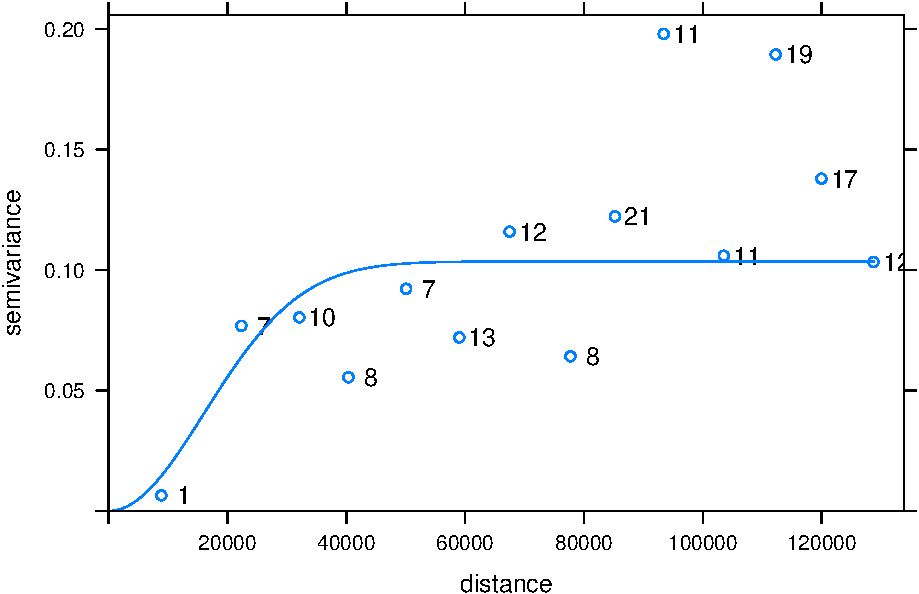
\includegraphics[width=800px]{Proyecto-Precipitaciones_files/figure-latex/vgm-pre1990-ajus-exp-3}

\begin{Shaded}
\begin{Highlighting}[]
\KeywordTok{attr}\NormalTok{(v90_m, }\StringTok{'SSErr'}\NormalTok{)}
\end{Highlighting}
\end{Shaded}

\begin{verbatim}
## [1] 4.207941e-11
\end{verbatim}

\begin{Shaded}
\begin{Highlighting}[]
\KeywordTok{attr}\NormalTok{(v90_m2, }\StringTok{'SSErr'}\NormalTok{) }\CommentTok{#Elegimos este}
\end{Highlighting}
\end{Shaded}

\begin{verbatim}
## [1] 3.619441e-11
\end{verbatim}

\begin{Shaded}
\begin{Highlighting}[]
\KeywordTok{attr}\NormalTok{(v90_m3, }\StringTok{'SSErr'}\NormalTok{)}
\end{Highlighting}
\end{Shaded}

\begin{verbatim}
## [1] 4.445952e-11
\end{verbatim}

\subsubsection{Interpolación por kriging
ordinario}\label{interpolaciuxf3n-por-kriging-ordinario}

Antes de realizar la interpolación, necesitamos una cuadrícula que
``llenaremos'' con las predcciones. Creemos una cuadrícula para RD, en
este caso, de baja resolución, 10x10km:

\begin{Shaded}
\begin{Highlighting}[]
\KeywordTok{library}\NormalTok{(stars)}
\end{Highlighting}
\end{Shaded}

\begin{verbatim}
## Loading required package: abind
\end{verbatim}

\begin{Shaded}
\begin{Highlighting}[]
\NormalTok{grd <-}\StringTok{ }\KeywordTok{st_bbox}\NormalTok{(prov) }\OperatorTok
\StringTok{  }\KeywordTok{st_as_stars}\NormalTok{(}\DataTypeTok{dx =} \DecValTok{10000}\NormalTok{) }\OperatorTok\StringTok{ }\CommentTok{#10000 metros=10km de resolución espacial}
\StringTok{  }\KeywordTok{st_set_crs}\NormalTok{(crsdestino) }\OperatorTok
\StringTok{  }\KeywordTok{st_crop}\NormalTok{(prov)}
\NormalTok{grd}
\end{Highlighting}
\end{Shaded}

\begin{verbatim}
## stars object with 2 dimensions and 1 attribute
## attribute(s):
##     values    
##  Min.   :0    
##  1st Qu.:0    
##  Median :0    
##  Mean   :0    
##  3rd Qu.:0    
##  Max.   :0    
##  NA's   :605  
## dimension(s):
##   from to  offset  delta                       refsys point values    
## x    1 39  182216  10000 +proj=utm +zone=19 +datum...    NA   NULL [x]
## y    1 28 2205216 -10000 +proj=utm +zone=19 +datum...    NA   NULL [y]
\end{verbatim}

\begin{Shaded}
\begin{Highlighting}[]
\KeywordTok{plot}\NormalTok{(grd)}
\end{Highlighting}
\end{Shaded}

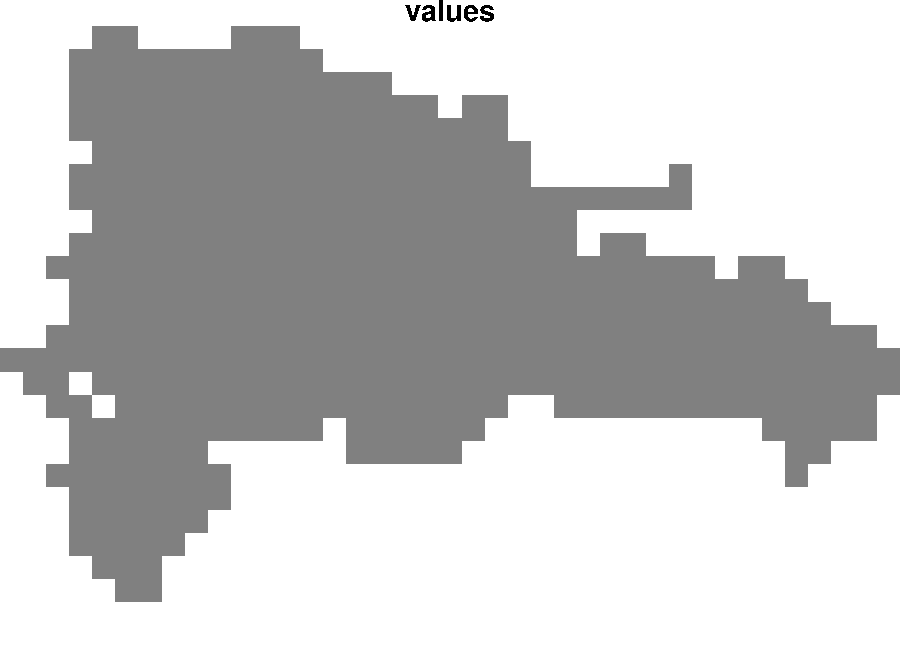
\includegraphics[width=800px]{Proyecto-Precipitaciones_files/figure-latex/grd-1}

Sobre ella, ejecutamos la interpolación por kriging ordinario. La
función \texttt{krige} asume que se trata de kriging ordinario, dado que
no se especifica un valor para el argumento \texttt{beta}, o media.

\begin{Shaded}
\begin{Highlighting}[]
\NormalTok{k <-}\StringTok{ }\KeywordTok{krige}\NormalTok{(}\DataTypeTok{formula =}\NormalTok{ a1990log}\OperatorTok{~}\DecValTok{1}\NormalTok{, }\DataTypeTok{locations =}\NormalTok{ pre1990, }\DataTypeTok{newdata =}\NormalTok{ grd, }\DataTypeTok{model =}\NormalTok{ v90_m2)}
\end{Highlighting}
\end{Shaded}

\begin{verbatim}
## [using ordinary kriging]
\end{verbatim}

\begin{Shaded}
\begin{Highlighting}[]
\NormalTok{k}
\end{Highlighting}
\end{Shaded}

\begin{verbatim}
## stars object with 2 dimensions and 2 attributes
## attribute(s):
##    var1.pred       var1.var      
##  Min.   :6.352   Min.   :0.0092  
##  1st Qu.:6.991   1st Qu.:0.0551  
##  Median :7.164   Median :0.0768  
##  Mean   :7.159   Mean   :0.0766  
##  3rd Qu.:7.343   3rd Qu.:0.0974  
##  Max.   :7.685   Max.   :0.1425  
##  NA's   :605     NA's   :605     
## dimension(s):
##   from to  offset  delta                       refsys point values    
## x    1 39  182216  10000 +proj=utm +zone=19 +datum...    NA   NULL [x]
## y    1 28 2205216 -10000 +proj=utm +zone=19 +datum...    NA   NULL [y]
\end{verbatim}

El objeto \texttt{k} es un ráster \texttt{stars} con dos variables,
\texttt{var1.pred} y \texttt{var1.var}, que son, respectivamente, la
predicción y la varianza de la predicción. La función \texttt{plot}
contiene un método para imprimir el objeto \texttt{k}.

\begin{Shaded}
\begin{Highlighting}[]
\KeywordTok{plot}\NormalTok{(k)}
\end{Highlighting}
\end{Shaded}

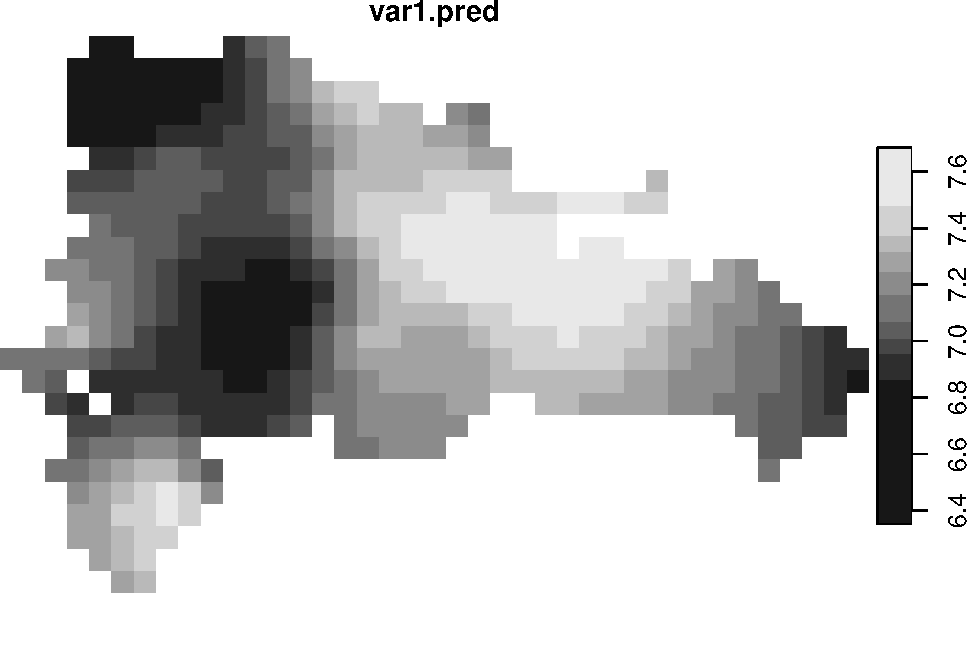
\includegraphics[width=800px]{Proyecto-Precipitaciones_files/figure-latex/krige-plot-raw-1}

Utilicemos \texttt{ggplot} para representar el objeto \texttt{stars}.

\begin{Shaded}
\begin{Highlighting}[]
\KeywordTok{ggplot}\NormalTok{() }\OperatorTok{+}
\StringTok{  }\KeywordTok{geom_stars}\NormalTok{(}\DataTypeTok{data =}\NormalTok{ k, }\KeywordTok{aes}\NormalTok{(}\DataTypeTok{fill =}\NormalTok{ var1.pred, }\DataTypeTok{x =}\NormalTok{ x, }\DataTypeTok{y =}\NormalTok{ y)) }\OperatorTok{+}\StringTok{ }
\StringTok{  }\KeywordTok{scale_fill_gradient}\NormalTok{(}\DataTypeTok{low=}\StringTok{"#deebf7"}\NormalTok{, }\DataTypeTok{high=}\StringTok{"#3182bd"}\NormalTok{) }\OperatorTok{+}
\StringTok{  }\KeywordTok{geom_sf}\NormalTok{(}\DataTypeTok{data =} \KeywordTok{st_cast}\NormalTok{(prov, }\StringTok{"MULTILINESTRING"}\NormalTok{)) }\OperatorTok{+}
\StringTok{  }\KeywordTok{geom_sf}\NormalTok{(}\DataTypeTok{data =}\NormalTok{ pre1990) }\OperatorTok{+}
\StringTok{  }\KeywordTok{geom_sf_text}\NormalTok{(}\DataTypeTok{data =}\NormalTok{ prov, }\KeywordTok{aes}\NormalTok{(}\DataTypeTok{label=}\NormalTok{TOPONIMIA), }\DataTypeTok{check_overlap =}\NormalTok{ T, }\DataTypeTok{size =} \DecValTok{2}\NormalTok{) }\OperatorTok{+}
\StringTok{  }\KeywordTok{theme_bw}\NormalTok{()}
\end{Highlighting}
\end{Shaded}

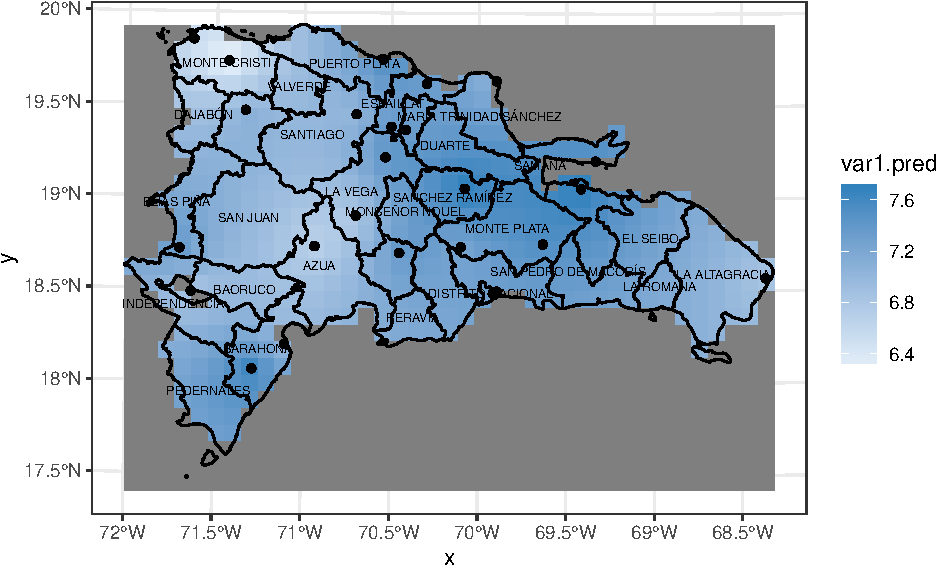
\includegraphics{Proyecto-Precipitaciones_files/figure-latex/krige-log-1.pdf}

Nótese en la leyenda que el objeto \texttt{k}, variable
\texttt{var1.pred} contiene las predicciones del logaritmo de la
precipitación para la cuadrícula de 10x10km (de ahí que el rango de la
leyenda sea \texttt{6.8-8.0}). Si calculamos \emph{e6.8} obtendremos el
valor de precipitación del límite inferior, y si calculamos \emph{e8}
obtendremos el límite superior.

Si queremos representar los valores de precipitación, debemos realizar
la operación inversa, que sería elevar al \texttt{e} el valor predicho
en \texttt{k}, lo cual se realiza mediante la función \texttt{exp()}.

\begin{Shaded}
\begin{Highlighting}[]
\KeywordTok{ggplot}\NormalTok{() }\OperatorTok{+}
\StringTok{  }\KeywordTok{geom_stars}\NormalTok{(}\DataTypeTok{data =} \KeywordTok{exp}\NormalTok{(k), }\KeywordTok{aes}\NormalTok{(}\DataTypeTok{fill =}\NormalTok{ var1.pred, }\DataTypeTok{x =}\NormalTok{ x, }\DataTypeTok{y =}\NormalTok{ y)) }\OperatorTok{+}\StringTok{ }
\StringTok{  }\KeywordTok{scale_fill_gradient}\NormalTok{(}\DataTypeTok{low=}\StringTok{"#deebf7"}\NormalTok{, }\DataTypeTok{high=}\StringTok{"#3182bd"}\NormalTok{, }\DataTypeTok{trans =} \StringTok{'log10'}\NormalTok{) }\OperatorTok{+}
\StringTok{  }\KeywordTok{geom_sf}\NormalTok{(}\DataTypeTok{data =} \KeywordTok{st_cast}\NormalTok{(prov, }\StringTok{"MULTILINESTRING"}\NormalTok{)) }\OperatorTok{+}
\StringTok{  }\KeywordTok{geom_sf}\NormalTok{(}\DataTypeTok{data =}\NormalTok{ pre1990) }\OperatorTok{+}
\StringTok{  }\KeywordTok{geom_sf_text}\NormalTok{(}\DataTypeTok{data =}\NormalTok{ prov, }\KeywordTok{aes}\NormalTok{(}\DataTypeTok{label=}\NormalTok{TOPONIMIA), }\DataTypeTok{check_overlap =}\NormalTok{ T, }\DataTypeTok{size =} \DecValTok{2}\NormalTok{) }\OperatorTok{+}
\StringTok{  }\KeywordTok{theme_bw}\NormalTok{()}
\end{Highlighting}
\end{Shaded}

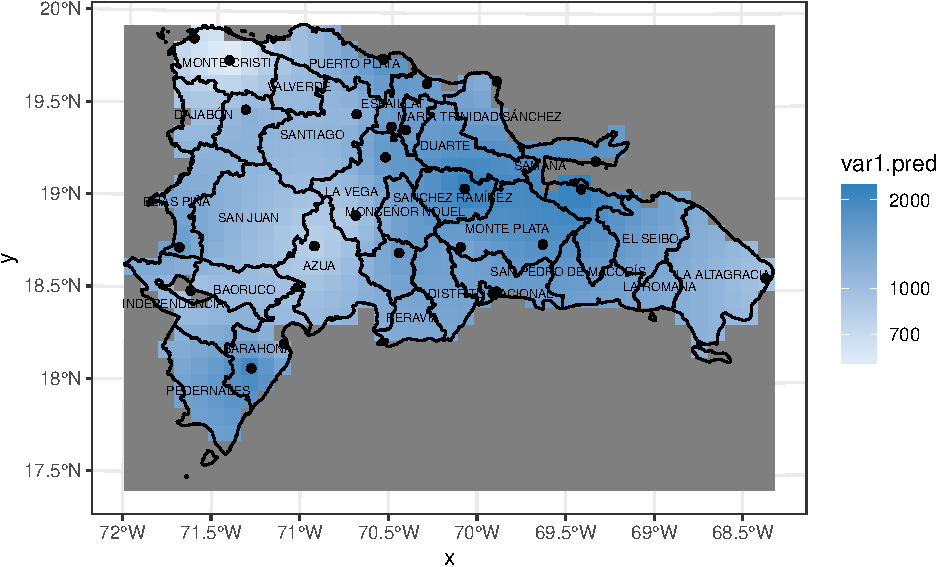
\includegraphics{Proyecto-Precipitaciones_files/figure-latex/krige-1.pdf}

\subsection{Estudio de caso: temperatura de República Dominicana
mediante kriging
universal}\label{estudio-de-caso-temperatura-de-repuxfablica-dominicana-mediante-kriging-universal}

Hasta este punto, logramos ejecutar un kriging ordinario para predecir
el valor de la precipitación de 1990 para todo el país a partir de 21
observatorios. Notemos que se trataba de un kriging ordinario, porque a
la función \texttt{krige} no le introducimos una media (argumento
\texttt{beta}), e igualmente porque con la función \texttt{variogram}
generamos un variograma contra un intercepto (fórmula
\texttt{a1990log\textasciitilde{}1}).

El kriging universal predice el valor de la variable de interés en
función del modelo espacial aportado por el variograma Y, al mismo
tiempo, considerando covariables mediante polinomios. En este ejemplo,
tomaremos la temperatura registrada en observatorios de ONAMET.

\subsubsection{Datos fuente}\label{datos-fuente-1}

\begin{Shaded}
\begin{Highlighting}[]
\NormalTok{rutatemp <-}\StringTok{ 'data/onamet_temp_anual.gpkg'}
\KeywordTok{st_layers}\NormalTok{(rutatemp)}
\end{Highlighting}
\end{Shaded}

\begin{verbatim}
## Driver: GPKG 
## Available layers:
##          layer_name geometry_type features fields
## 1 onamet_temp_anual         Point       72     14
\end{verbatim}

\begin{Shaded}
\begin{Highlighting}[]
\NormalTok{temp <-}\StringTok{ }\KeywordTok{st_read}\NormalTok{(rutatemp)}
\end{Highlighting}
\end{Shaded}

\begin{verbatim}
## Reading layer `onamet_temp_anual' from data source `/home/rober/unidad-0-asignacion-99-mi-proyecto/data/onamet_temp_anual.gpkg' using driver `GPKG'
## Simple feature collection with 72 features and 14 fields
## geometry type:  POINT
## dimension:      XY
## bbox:           xmin: 199028.4 ymin: 1967717 xmax: 566825.1 ymax: 2199684
## epsg (SRID):    32619
## proj4string:    +proj=utm +zone=19 +datum=WGS84 +units=m +no_defs
\end{verbatim}

\begin{Shaded}
\begin{Highlighting}[]
\NormalTok{temp}
\end{Highlighting}
\end{Shaded}

\begin{verbatim}
## Simple feature collection with 72 features and 14 fields
## geometry type:  POINT
## dimension:      XY
## bbox:           xmin: 199028.4 ymin: 1967717 xmax: 566825.1 ymax: 2199684
## epsg (SRID):    32619
## proj4string:    +proj=utm +zone=19 +datum=WGS84 +units=m +no_defs
## First 10 features:
##           nombre  ene  feb  mar  abr  may  jun  jul  ago  sep  oct  nov
## 1        HERRERA 24.6 24.4 24.8 25.8 26.4 27.1 27.4 27.4 27.1 26.9 26.1
## 2       LA UNION 23.3 23.3 23.8 24.7 25.7 27.0 27.0 27.1 26.9 26.3 25.0
## 3  ARROYO BARRIL 24.6 24.9 25.6 26.1 26.4 27.1 27.1 26.8 26.8 26.6 25.7
## 4           AZUA 25.2 25.5 26.2 26.8 27.3 27.7 28.4 28.5 28.1 27.4 26.6
## 5           BANI 25.9 26.0 26.7 27.4 27.6 27.9 28.6 28.5 28.1 27.6 27.0
## 6       BARAHONA 24.6 24.8 25.4 26.2 26.7 27.3 27.9 27.9 27.5 26.7 26.2
## 7      BAYAGUANA 24.6 24.9 25.6 26.3 27.0 27.6 27.7 27.6 27.5 27.2 26.3
## 8          BONAO 23.4 23.8 24.6 25.4 25.9 26.8 26.9 27.0 26.8 26.4 25.2
## 9        CABRERA 24.7 24.8 25.2 25.6 26.0 26.6 26.8 26.8 26.7 26.5 25.7
## 10       CEVICOS 23.0 23.4 24.3 25.2 26.0 26.6 26.6 26.6 26.6 26.1 24.7
##     dic tanual                     geom
## 1  25.1   26.1 POINT (397885.6 2042020)
## 2  23.7   25.3 POINT (337547.6 2184493)
## 3  25.0   26.1 POINT (452651.8 2124797)
## 4  25.5   26.9 POINT (316911.7 2040776)
## 5  25.9   27.3 POINT (359011.1 2020133)
## 6  25.2   26.4 POINT (277856.2 2013510)
## 7  25.0   26.4 POINT (433198.1 2073212)
## 8  23.8   25.5 POINT (352534.2 2093960)
## 9  24.9   25.9 POINT (405589.5 2171085)
## 10 23.3   25.2 POINT (398204.6 2101037)
\end{verbatim}

Exploremos el CRS del objeto \texttt{obs}.

\begin{Shaded}
\begin{Highlighting}[]
\KeywordTok{st_crs}\NormalTok{(temp)}
\end{Highlighting}
\end{Shaded}

\begin{verbatim}
## Coordinate Reference System:
##   EPSG: 32619 
##   proj4string: "+proj=utm +zone=19 +datum=WGS84 +units=m +no_defs"
\end{verbatim}

Dado que es EPSG:32619 no necesitamos realizar transformación alguna.

\subsubsection{EDA básico}\label{eda-buxe1sico-1}

Obtengamos los estadísticos básicos del objeto \texttt{temp} y de su
variable \texttt{tanual}:

\begin{Shaded}
\begin{Highlighting}[]
\KeywordTok{nrow}\NormalTok{(temp)}
\end{Highlighting}
\end{Shaded}

\begin{verbatim}
## [1] 72
\end{verbatim}

\begin{Shaded}
\begin{Highlighting}[]
\KeywordTok{summary}\NormalTok{(temp}\OperatorTok{$}\NormalTok{tanual)}
\end{Highlighting}
\end{Shaded}

\begin{verbatim}
##    Min. 1st Qu.  Median    Mean 3rd Qu.    Max. 
##   18.20   25.20   25.90   25.50   26.43   28.40
\end{verbatim}

\begin{Shaded}
\begin{Highlighting}[]
\KeywordTok{hist}\NormalTok{(temp}\OperatorTok{$}\NormalTok{tanual)}
\end{Highlighting}
\end{Shaded}

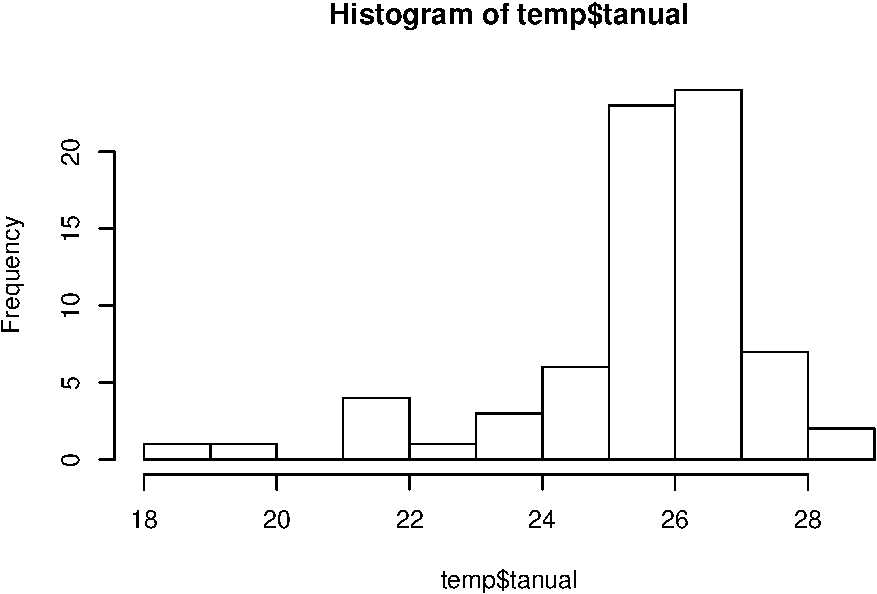
\includegraphics[width=600px]{Proyecto-Precipitaciones_files/figure-latex/esda-temp-1}

\begin{Shaded}
\begin{Highlighting}[]
\KeywordTok{qqnorm}\NormalTok{(temp}\OperatorTok{$}\NormalTok{tanual)}
\end{Highlighting}
\end{Shaded}

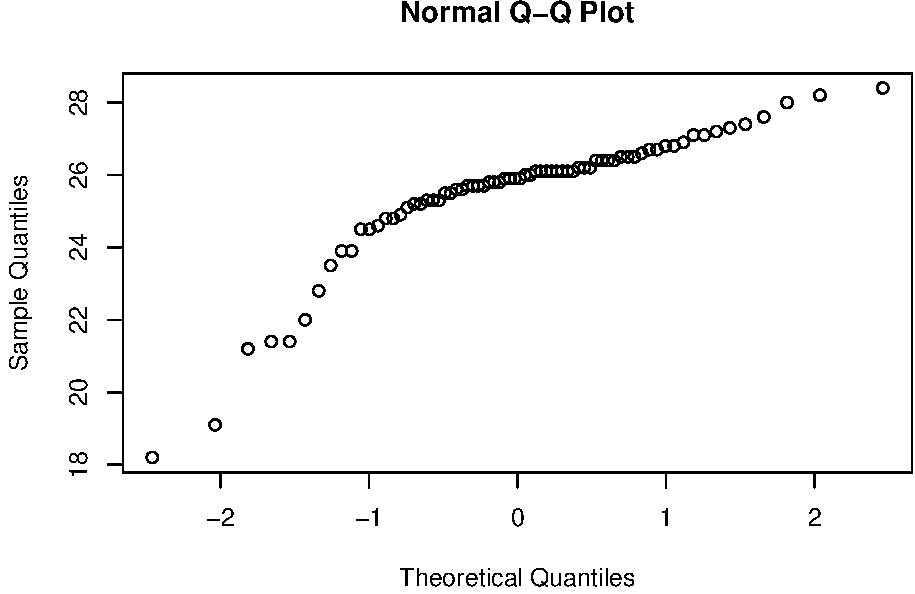
\includegraphics[width=600px]{Proyecto-Precipitaciones_files/figure-latex/esda-temp-2}

\begin{Shaded}
\begin{Highlighting}[]
\KeywordTok{hist}\NormalTok{(}\KeywordTok{log}\NormalTok{(temp}\OperatorTok{$}\NormalTok{tanual))}
\end{Highlighting}
\end{Shaded}

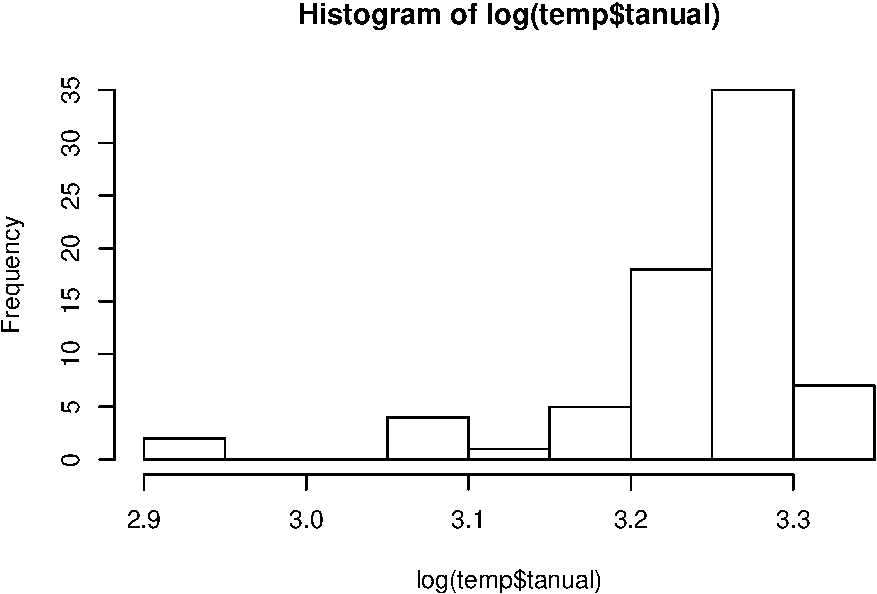
\includegraphics[width=600px]{Proyecto-Precipitaciones_files/figure-latex/esda-temp-3}

\begin{Shaded}
\begin{Highlighting}[]
\KeywordTok{qqnorm}\NormalTok{(}\KeywordTok{log}\NormalTok{(temp}\OperatorTok{$}\NormalTok{tanual))}
\end{Highlighting}
\end{Shaded}

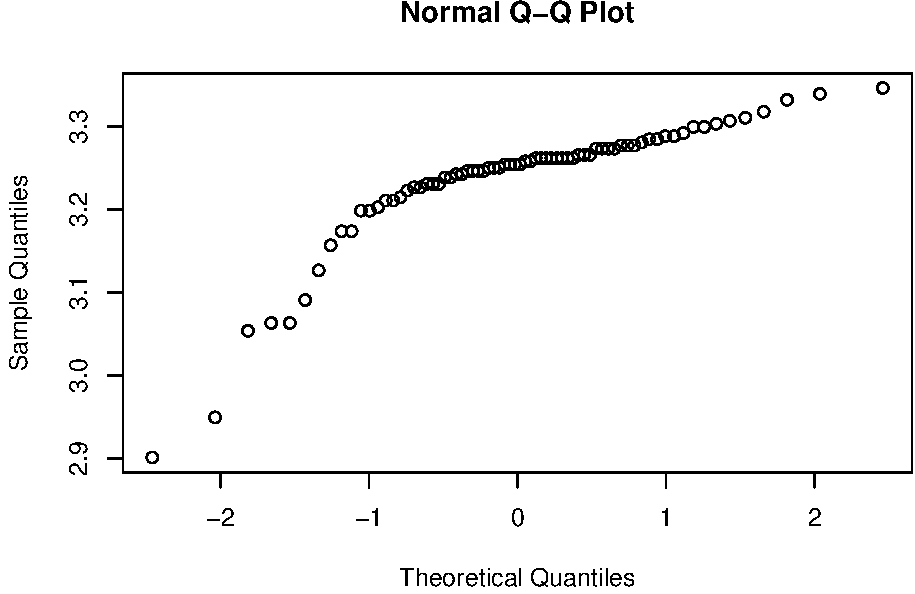
\includegraphics[width=600px]{Proyecto-Precipitaciones_files/figure-latex/esda-temp-4}

\begin{Shaded}
\begin{Highlighting}[]
\KeywordTok{shapiro.test}\NormalTok{(temp}\OperatorTok{$}\NormalTok{tanual)}
\end{Highlighting}
\end{Shaded}

\begin{verbatim}
## 
##  Shapiro-Wilk normality test
## 
## data:  temp$tanual
## W = 0.81613, p-value = 4.783e-08
\end{verbatim}

\begin{Shaded}
\begin{Highlighting}[]
\KeywordTok{shapiro.test}\NormalTok{(}\KeywordTok{log}\NormalTok{(temp}\OperatorTok{$}\NormalTok{tanual))}
\end{Highlighting}
\end{Shaded}

\begin{verbatim}
## 
##  Shapiro-Wilk normality test
## 
## data:  log(temp$tanual)
## W = 0.77059, p-value = 3e-09
\end{verbatim}

Dado que en este caso existe una fuerte desviación de una distribución
normal, debemos tenerlo en cuenta al modelizar la temperatura respecto
de la elevación. Al menos los residuos deberían tener distribución
normal. Exploraremos el modelo oportunamente. Visualicemos los datos en
un mapa

\begin{Shaded}
\begin{Highlighting}[]
\KeywordTok{library}\NormalTok{(RColorBrewer)}
\KeywordTok{ggplot}\NormalTok{() }\OperatorTok{+}
\StringTok{  }\KeywordTok{geom_sf}\NormalTok{(}\DataTypeTok{data =}\NormalTok{ prov, }\DataTypeTok{fill =} \StringTok{'white'}\NormalTok{) }\OperatorTok{+}
\StringTok{  }\KeywordTok{geom_sf}\NormalTok{(}\DataTypeTok{data =}\NormalTok{ temp, }\KeywordTok{aes}\NormalTok{(}\DataTypeTok{col =}\NormalTok{ tanual), }\DataTypeTok{size =} \DecValTok{6}\NormalTok{) }\OperatorTok{+}\StringTok{ }
\StringTok{  }\KeywordTok{scale_colour_gradientn}\NormalTok{(}\DataTypeTok{colours =} \KeywordTok{rev}\NormalTok{(}\KeywordTok{brewer.pal}\NormalTok{(}\DecValTok{9}\NormalTok{, }\DataTypeTok{name =} \StringTok{'RdBu'}\NormalTok{))) }\OperatorTok{+}
\StringTok{  }\KeywordTok{geom_sf_text}\NormalTok{(}\DataTypeTok{data =}\NormalTok{ temp, }\KeywordTok{aes}\NormalTok{(}\DataTypeTok{label=}\NormalTok{nombre), }\DataTypeTok{check_overlap =}\NormalTok{ T, }\DataTypeTok{size =} \FloatTok{1.5}\NormalTok{) }\OperatorTok{+}
\StringTok{  }\KeywordTok{theme_bw}\NormalTok{()}
\end{Highlighting}
\end{Shaded}

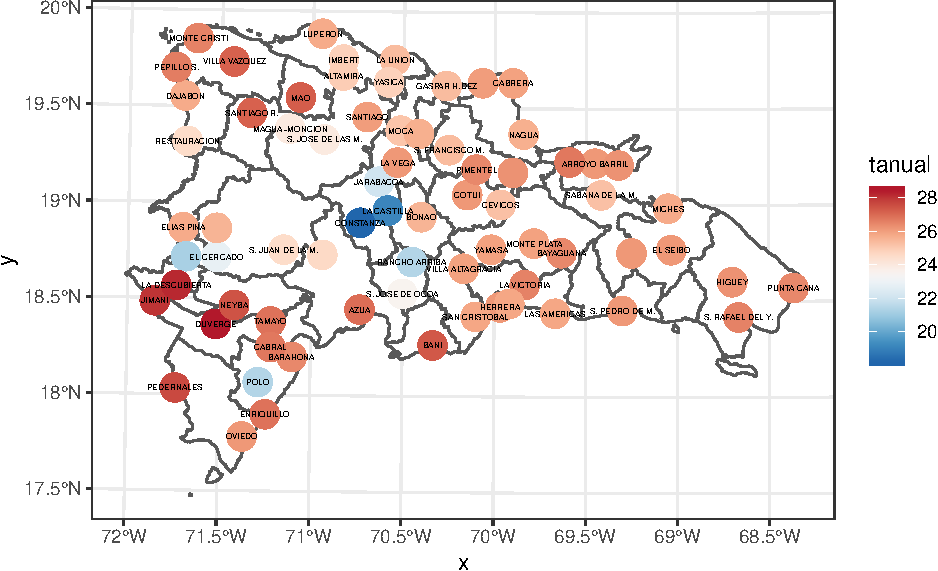
\includegraphics{Proyecto-Precipitaciones_files/figure-latex/mapa-temp-1.pdf}

\subsubsection{Importar DEM}\label{importar-dem}

Ahora necesitamos traer el DEM, que en este caso será uno resumido a
partir del SRTM-90m.

\begin{Shaded}
\begin{Highlighting}[]
\NormalTok{dem <-}\StringTok{ }\KeywordTok{read_stars}\NormalTok{(}\StringTok{'data/dem_srtm_remuestreado.tif'}\NormalTok{)}
\KeywordTok{names}\NormalTok{(dem) <-}\StringTok{ 'ele'}
\KeywordTok{plot}\NormalTok{(dem)}
\end{Highlighting}
\end{Shaded}

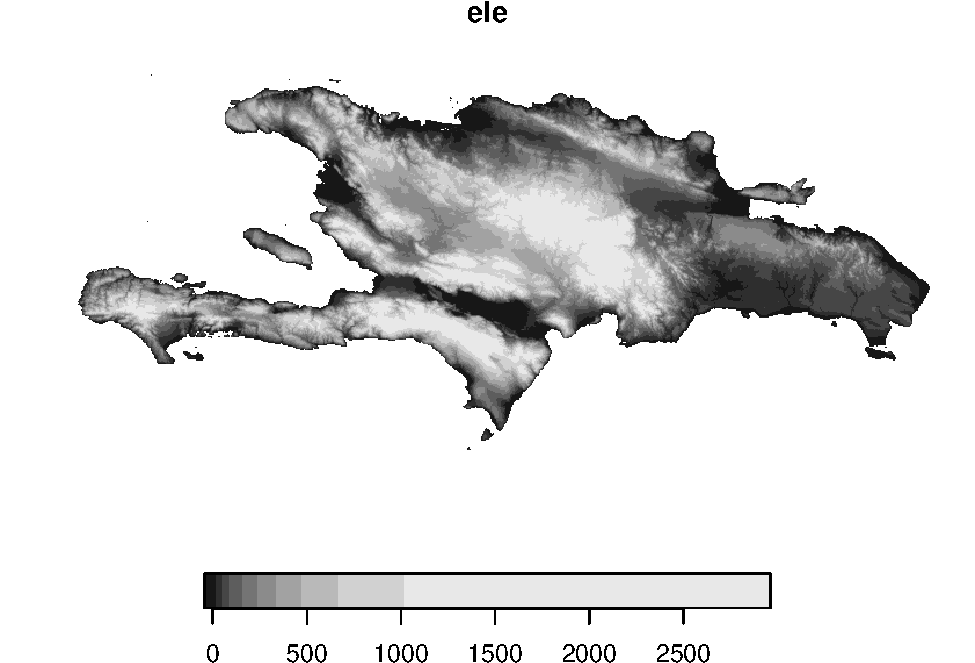
\includegraphics[width=800px]{Proyecto-Precipitaciones_files/figure-latex/dem-1}

Ahora remuestreamos el DEM para que se alinee con la cuadrícula fuente,
\texttt{grd}. El DEM remuestreado será la cuadrícula del covariable
(variable independiente) que utilizaremos para predecir el valor de
temperatura.

\begin{Shaded}
\begin{Highlighting}[]
\NormalTok{grdcovars <-}\StringTok{ }\KeywordTok{aggregate}\NormalTok{(dem, grd, mean, }\DataTypeTok{na.rm=}\NormalTok{T)}
\KeywordTok{plot}\NormalTok{(grdcovars)}
\end{Highlighting}
\end{Shaded}

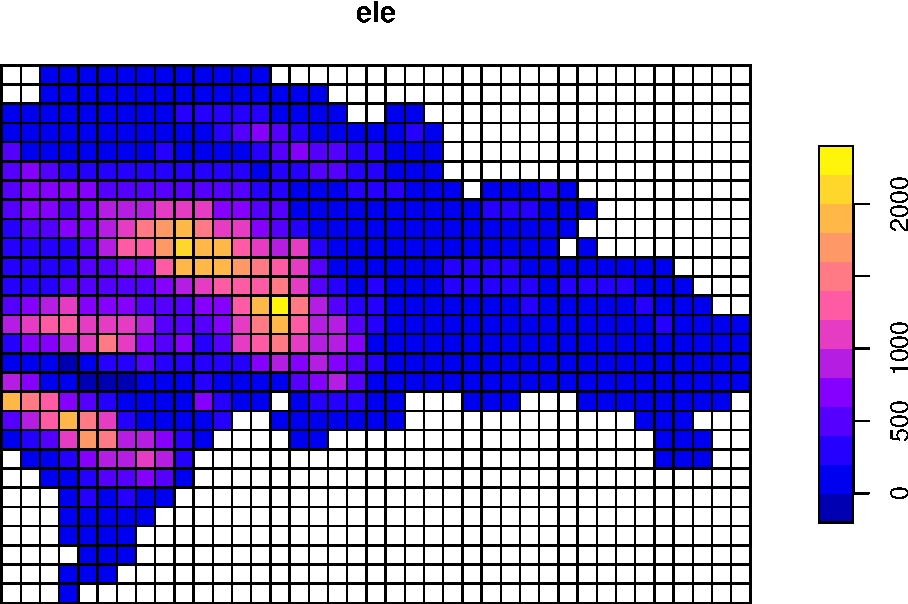
\includegraphics[width=800px]{Proyecto-Precipitaciones_files/figure-latex/remuestrear-dem-1}

\subsubsection{Extraer datos de elevación y generar
modelo}\label{extraer-datos-de-elevaciuxf3n-y-generar-modelo}

Necesitamos que los datos de elevación pasen al objeto \texttt{temp}, de
manera que podamos probar un modelo lineal que ponga en relación a la
elevación con la temperatura.

\begin{Shaded}
\begin{Highlighting}[]
\NormalTok{temp}\OperatorTok{$}\NormalTok{ele <-}\StringTok{ }\KeywordTok{st_as_sf}\NormalTok{(}\KeywordTok{aggregate}\NormalTok{(grdcovars, temp, mean))[[}\DecValTok{1}\NormalTok{]]}
\NormalTok{temp}\OperatorTok{$}\NormalTok{ele}
\end{Highlighting}
\end{Shaded}

\begin{verbatim}
##  [1]   37.04137  111.19428   96.23608   89.05470   53.63334  360.12991
##  [7]   49.84021  235.65909   83.14058  155.80394 1373.07323   57.56667
## [13]   82.44868  218.63500 1042.68780  122.73364  419.19694  151.41004
## [19]   94.38337   79.46646  115.23488 1355.50136  945.64083   66.49686
## [25] 1152.72653   29.14500  165.08992   24.01264   21.70497  443.20785
## [31]   41.29578  108.17977  167.63144   25.13954   66.00372   56.24511
## [37]   -4.08697   50.94419   10.78244  140.73771   41.89802 1010.59454
## [43]   11.03355  879.47538  617.60780   84.08008   14.71723  157.90341
## [49]   99.80911   58.09217  489.49667  647.02488   61.22240  212.92748
## [55]  191.10207   29.83365   24.18545  181.29521   79.46121  241.98926
## [61]  498.26058  529.88060   11.89785   53.39107   22.52430   26.70314
## [67]  237.12488   44.10347   72.15647  271.38220         NA  690.64947
\end{verbatim}

\begin{Shaded}
\begin{Highlighting}[]
\NormalTok{temp <-}\StringTok{ }\NormalTok{temp[}\OperatorTok{!}\KeywordTok{is.na}\NormalTok{(temp}\OperatorTok{$}\NormalTok{ele),] }\CommentTok{#Quitar observación con NA}
\KeywordTok{plot}\NormalTok{(temp}\OperatorTok{$}\NormalTok{tanual, temp}\OperatorTok{$}\NormalTok{ele)}
\end{Highlighting}
\end{Shaded}

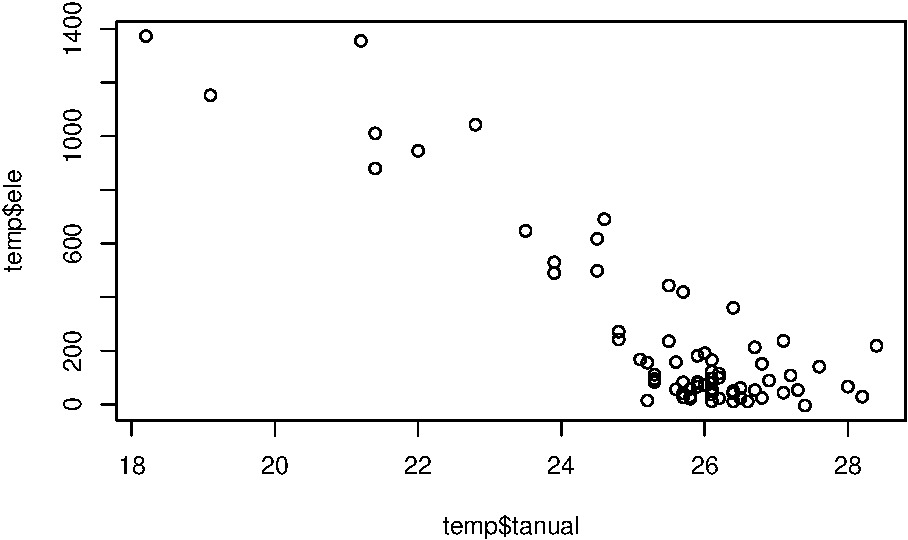
\includegraphics[width=600px]{Proyecto-Precipitaciones_files/figure-latex/agregar-y-modelo-1}

\begin{Shaded}
\begin{Highlighting}[]
\NormalTok{temp_lm <-}\StringTok{ }\KeywordTok{lm}\NormalTok{(tanual }\OperatorTok{~}\StringTok{ }\NormalTok{ele, temp)}
\KeywordTok{summary}\NormalTok{(temp_lm)}
\end{Highlighting}
\end{Shaded}

\begin{verbatim}
## 
## Call:
## lm(formula = tanual ~ ele, data = temp)
## 
## Residuals:
##     Min      1Q  Median      3Q     Max 
## -1.9474 -0.5766 -0.1059  0.6037  2.7525 
## 
## Coefficients:
##              Estimate Std. Error t value Pr(>|t|)    
## (Intercept) 26.724159   0.129657  206.11   <2e-16 ***
## ele         -0.004925   0.000314  -15.68   <2e-16 ***
## ---
## Signif. codes:  0 '***' 0.001 '**' 0.01 '*' 0.05 '.' 0.1 ' ' 1
## 
## Residual standard error: 0.8768 on 69 degrees of freedom
## Multiple R-squared:  0.7809, Adjusted R-squared:  0.7777 
## F-statistic: 245.9 on 1 and 69 DF,  p-value: < 2.2e-16
\end{verbatim}

\begin{Shaded}
\begin{Highlighting}[]
\KeywordTok{plot}\NormalTok{(temp_lm)}
\end{Highlighting}
\end{Shaded}

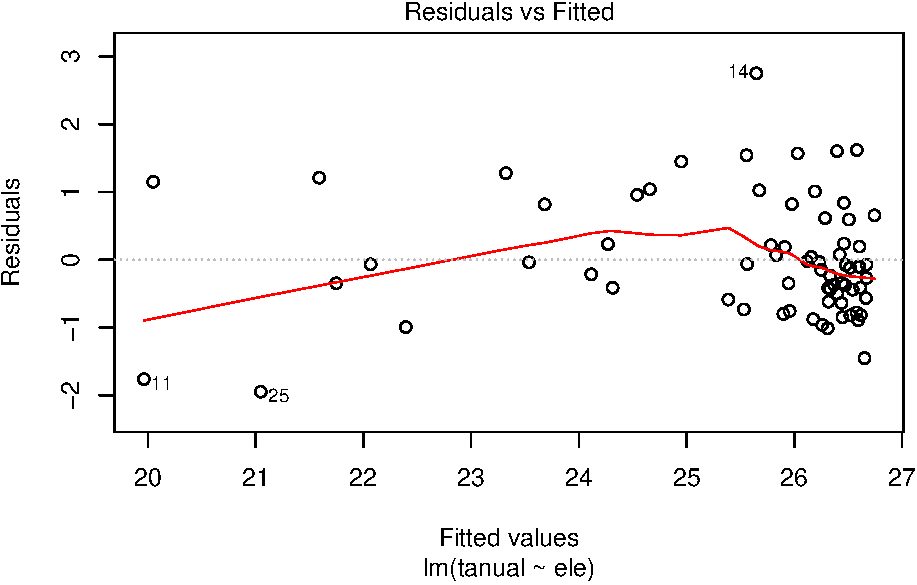
\includegraphics[width=600px]{Proyecto-Precipitaciones_files/figure-latex/agregar-y-modelo-2}
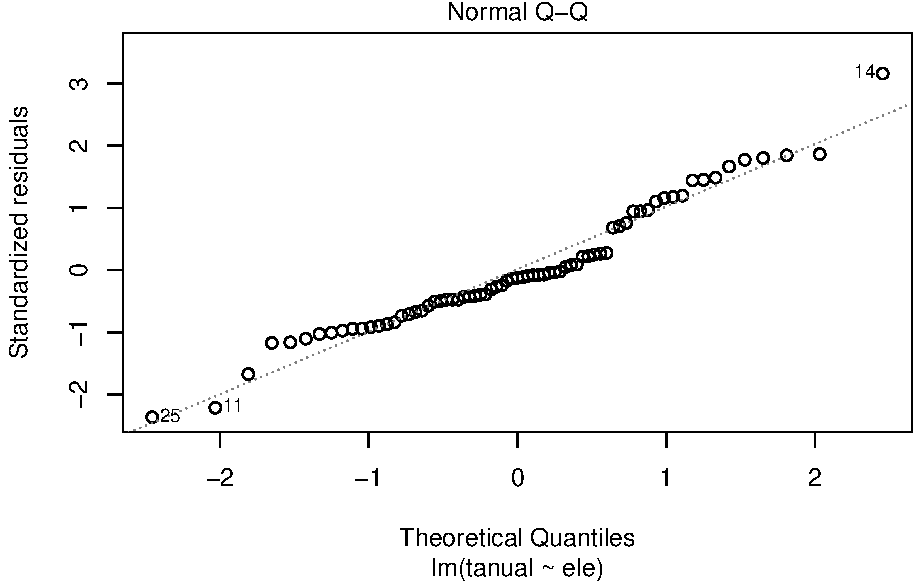
\includegraphics[width=600px]{Proyecto-Precipitaciones_files/figure-latex/agregar-y-modelo-3}
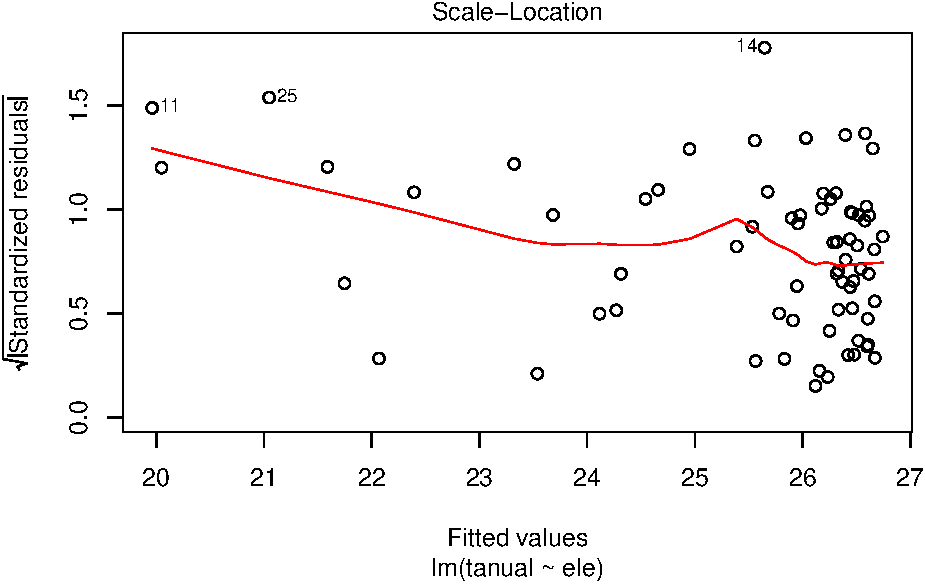
\includegraphics[width=600px]{Proyecto-Precipitaciones_files/figure-latex/agregar-y-modelo-4}
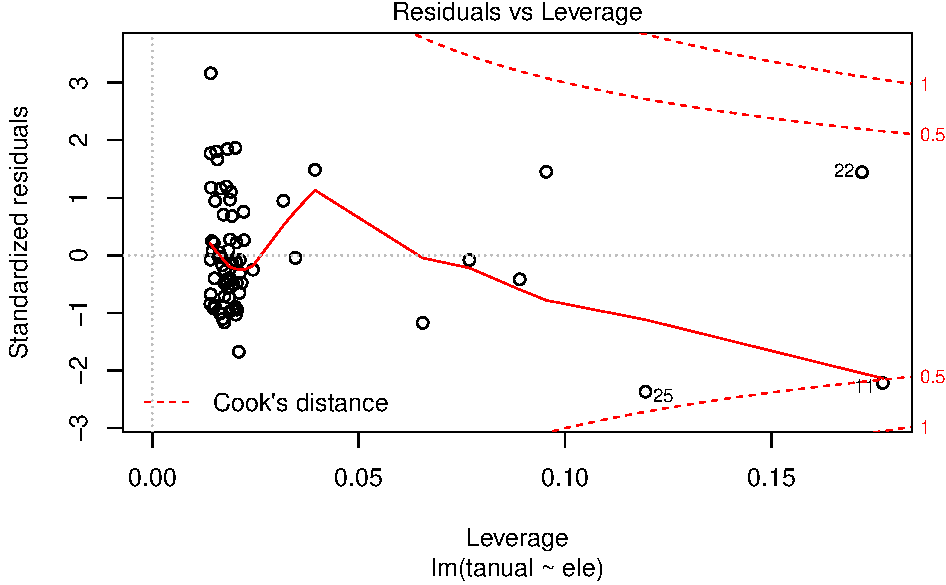
\includegraphics[width=600px]{Proyecto-Precipitaciones_files/figure-latex/agregar-y-modelo-5}

El modelo sugiere que existe asociación entre temperatura y elevación,
lo cual es esperable. En este caso, el gradiente resultante es de unos
-0.5°C por cada 100 metros de elevación. El gradiente comúnmente es de
-0.7°C/100m, pero en este caso, al utilizar un DEM resumido, el
gradiente igualmente se atenúa. Generemos variograma muestral con este
modelo.

\subsubsection{Variograma muestral}\label{variograma-muestral-1}

\begin{Shaded}
\begin{Highlighting}[]
\NormalTok{vt <-}\StringTok{ }\KeywordTok{variogram}\NormalTok{(tanual }\OperatorTok{~}\StringTok{ }\NormalTok{ele, temp)}
\NormalTok{vt}
\end{Highlighting}
\end{Shaded}

\begin{verbatim}
##     np       dist      gamma dir.hor dir.ver   id
## 1    1   5700.529 0.05627847       0       0 var1
## 2   32  16704.469 0.33635604       0       0 var1
## 3   48  24262.705 0.54374141       0       0 var1
## 4   71  33650.837 0.35356827       0       0 var1
## 5   95  43808.242 0.50038750       0       0 var1
## 6   96  53318.232 0.47861452       0       0 var1
## 7  119  63032.130 0.55137087       0       0 var1
## 8  114  72385.146 0.38117872       0       0 var1
## 9  117  82661.116 0.64274923       0       0 var1
## 10 132  91995.843 0.62593645       0       0 var1
## 11 121 101582.482 0.67431891       0       0 var1
## 12 133 111087.873 0.66429574       0       0 var1
## 13 127 120784.573 0.93949779       0       0 var1
## 14 137 130797.186 0.74052779       0       0 var1
## 15 119 140308.927 0.76607643       0       0 var1
\end{verbatim}

\begin{Shaded}
\begin{Highlighting}[]
\KeywordTok{plot}\NormalTok{(vt)}
\end{Highlighting}
\end{Shaded}

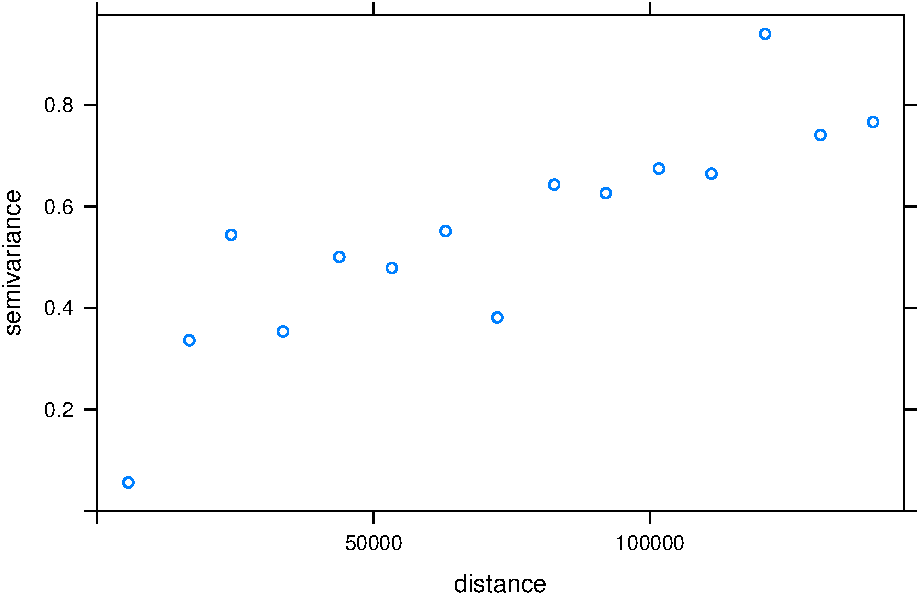
\includegraphics[width=800px]{Proyecto-Precipitaciones_files/figure-latex/vgm-temp-1}

\subsubsection{Variograma modelo}\label{variograma-modelo-1}

Parecería razonable utilizar un variograma modelo exponencial con rango
corto, por ejemplo, 20 o 30 km. Probemos.

\begin{Shaded}
\begin{Highlighting}[]
\NormalTok{vt_m <-}\StringTok{ }\KeywordTok{fit.variogram}\NormalTok{(vt, }\KeywordTok{vgm}\NormalTok{(}\DataTypeTok{model =} \StringTok{"Exp"}\NormalTok{, }\DataTypeTok{range =} \DecValTok{30000}\NormalTok{))}
\NormalTok{vt_m}
\end{Highlighting}
\end{Shaded}

\begin{verbatim}
##   model     psill   range
## 1   Exp 0.6121034 22069.9
\end{verbatim}

\begin{Shaded}
\begin{Highlighting}[]
\KeywordTok{plot}\NormalTok{(vt, vt_m, }\DataTypeTok{plot.numbers =}\NormalTok{ T)}
\end{Highlighting}
\end{Shaded}

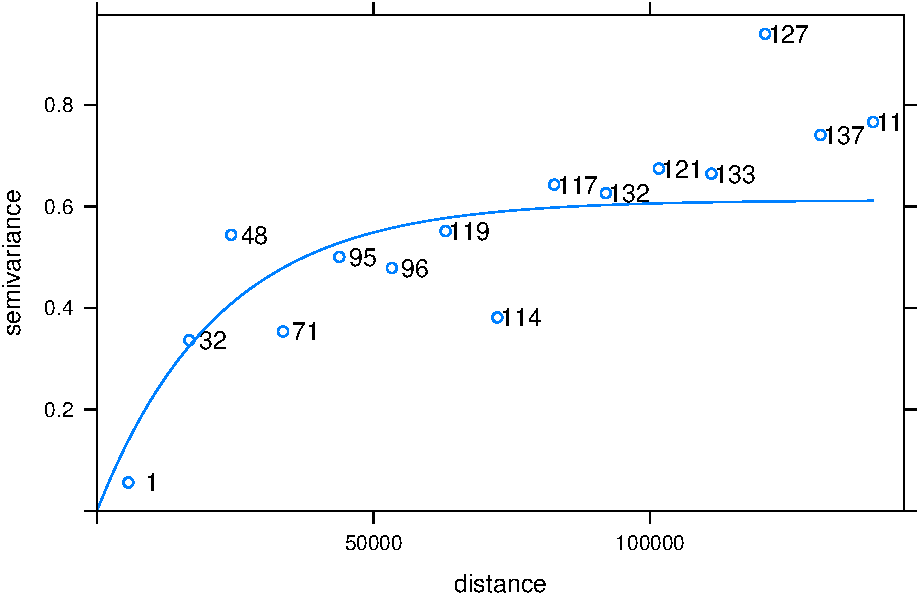
\includegraphics[width=800px]{Proyecto-Precipitaciones_files/figure-latex/vgm-temp-ajus-1}

\subsubsection{Kriging universal}\label{kriging-universal}

Finalmnente, ejecutamos el kriging.

\begin{Shaded}
\begin{Highlighting}[]
\NormalTok{k_u <-}\StringTok{ }\KeywordTok{krige}\NormalTok{(tanual }\OperatorTok{~}\StringTok{ }\NormalTok{ele, temp, }\KeywordTok{st_rasterize}\NormalTok{(}\KeywordTok{st_as_sf}\NormalTok{(grdcovars)), vt_m)}
\end{Highlighting}
\end{Shaded}

\begin{verbatim}
## [using universal kriging]
\end{verbatim}

Finalmente, lo representamos.

\begin{Shaded}
\begin{Highlighting}[]
\KeywordTok{ggplot}\NormalTok{() }\OperatorTok{+}
\StringTok{  }\KeywordTok{geom_stars}\NormalTok{(}\DataTypeTok{data =}\NormalTok{ k_u, }\KeywordTok{aes}\NormalTok{(}\DataTypeTok{fill =}\NormalTok{ var1.pred, }\DataTypeTok{x =}\NormalTok{ x, }\DataTypeTok{y =}\NormalTok{ y)) }\OperatorTok{+}\StringTok{ }
\StringTok{  }\KeywordTok{scale_fill_gradientn}\NormalTok{(}\DataTypeTok{colours =} \KeywordTok{rev}\NormalTok{(}\KeywordTok{brewer.pal}\NormalTok{(}\DecValTok{9}\NormalTok{, }\DataTypeTok{name =} \StringTok{'RdBu'}\NormalTok{))) }\OperatorTok{+}
\StringTok{  }\KeywordTok{geom_sf}\NormalTok{(}\DataTypeTok{data =} \KeywordTok{st_cast}\NormalTok{(prov, }\StringTok{"MULTILINESTRING"}\NormalTok{)) }\OperatorTok{+}
\StringTok{  }\KeywordTok{geom_sf}\NormalTok{(}\DataTypeTok{data =}\NormalTok{ pre1990) }\OperatorTok{+}
\StringTok{  }\KeywordTok{geom_sf_text}\NormalTok{(}\DataTypeTok{data =}\NormalTok{ prov, }\KeywordTok{aes}\NormalTok{(}\DataTypeTok{label=}\NormalTok{TOPONIMIA), }\DataTypeTok{check_overlap =}\NormalTok{ T, }\DataTypeTok{size =} \DecValTok{2}\NormalTok{) }\OperatorTok{+}
\StringTok{  }\KeywordTok{theme_bw}\NormalTok{()}
\end{Highlighting}
\end{Shaded}

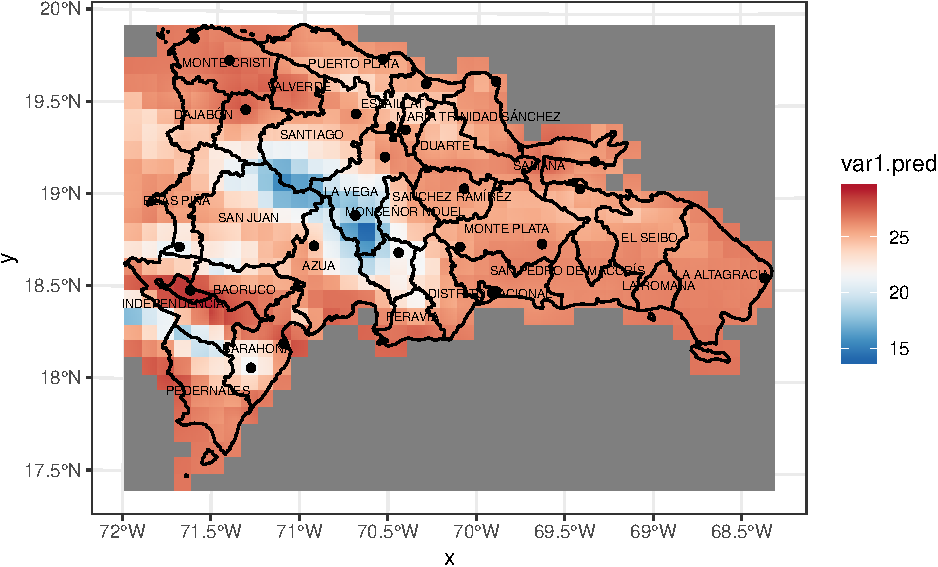
\includegraphics{Proyecto-Precipitaciones_files/figure-latex/krige-uk-1.pdf}

\subsubsection{Nota final}\label{nota-final}

Dado que en este caso existe una fuerte desviación de los datos respecto
a una distribución normal, aun usando transformación logarítmica, se
recomienda aplicar otro tipo de transformación. En este caso, luce mejor
emplear \emph{Tukey Ladder of Powers} (escalera de potencias de Tukey).
Usaremos la función \texttt{transformTukey} del paquete
\texttt{rcompanion}, que cargaremos a continuación.

\begin{Shaded}
\begin{Highlighting}[]
\KeywordTok{library}\NormalTok{(rcompanion)}
\NormalTok{temp}\OperatorTok{$}\NormalTok{tanualtrans <-}\StringTok{ }\KeywordTok{transformTukey}\NormalTok{(temp}\OperatorTok{$}\NormalTok{tanual, }\DataTypeTok{plotit =}\NormalTok{ F)}
\KeywordTok{hist}\NormalTok{(temp}\OperatorTok{$}\NormalTok{tanualtrans)}
\KeywordTok{qqnorm}\NormalTok{(temp}\OperatorTok{$}\NormalTok{tanualtrans)}
\KeywordTok{shapiro.test}\NormalTok{(temp}\OperatorTok{$}\NormalTok{tanualtrans)}
\end{Highlighting}
\end{Shaded}

\ldots

\section{Referencias}\label{referencias}




\newpage
\singlespacing 
\end{document}
